\documentclass[a4paper,12pt]{article}
\usepackage{epsfig,amssymb,amsmath,}
\usepackage{color}

\textwidth=18cm%6.25true in
\textheight=24.5cm%9.65true in
\voffset=-2.5cm%-1true in
\hoffset=-0.75true in

%%%%%%%%%%%%%%%%%%%%%%%%%%%%%%%%%%%%%%%%%%%%%%%%%%%%%%%%%%%%%%%%%%
%\usepackage[sorting=none, url=false, style=numeric-comp]{biblatex}
%\bibliography{../global.bib}
%%%%%%%%%%%%%%%%%%%%%%%%%%%%%%%%%%%%%%%%%%%%%%%%%%%%%%%%%%%%%%%%%%
\usepackage[sort&compress,numbers]{natbib}
\bibliographystyle{apsrev4-1}
\usepackage{doi}%<----------
% https://tex.stackexchange.com/questions/15677
%%%%%%%%%%%%%%%%%%%%%%%%%%%%%%%%%%%%%%%%%%%%%%%%%%%%%%%%%%%%%%%%%%

\usepackage{tikz}
\usetikzlibrary{arrows}
\usepackage[]{hyperref}     
%\hypersetup{citecolor = blue, linktocpage=true}
\usepackage{titlesec}
\titleformat{\subsection}
{\normalfont\large\bfseries}{\thesubsection}{1em}{}

\usepackage{graphicx} % Allows including images    
\graphicspath{{../figures/}, {../figures/growthrates/}}

\usepackage{dcolumn}
\usepackage{array}
\newcolumntype{P}[1]{>{\centering\arraybackslash}p{#1}}
\usepackage{makecell}

\renewcommand{\bf}{\mathbf}
\renewcommand{\cal}{\mathcal}
\newcommand{\pd}[2]{\frac{\partial #1}{\partial #2}}
\newcommand{\pdn}[3]{\frac{\partial^{#3} #1}{\partial #2^{#3}}}
\newcommand{\pdop}[1]{\frac{\partial}{\partial #1}}
\newcommand{\nd}[2]{\frac{d #1}{d #2}}
\newcommand{\ndn}[3]{\frac{d^{#3} #1}{d #2^{#3}}}
\newcommand{\ndop}[1]{\frac{d}{d #1}}
\newcommand{\dt}{\frac{d}{dt}}
\newcommand{\half}{\frac{1}{2}}
\newcommand{\third}{\frac{1}{3}}
\renewcommand{\th}[1]{\frac{1}{#1}}
\newcommand{\ex}[1]{\left\langle #1 \right\rangle}
\newcommand{\abs}[1]{\left| #1 \right|}
\renewcommand{\d}{\delta}
\renewcommand{\l}{\ell}
\renewcommand{\t}{\tau}
\renewcommand{\S}{\mathcal{S}}
\newcommand{\nc}{\text{nc}}
\newcommand{\ret}{\text{return}}
\newcommand{\tot}{\text{tot}}
\newcommand{\ket}[1]{\left|#1\right\rangle}
\newcommand{\bra}[1]{\left\langle#1\right|}
\newcommand{\braket}[2]{\left\langle#1\middle|#2\right\rangle}
\newcommand{\brakett}[3]{\left\langle#1\middle|#2\middle|#3\right\rangle}
\newcommand{\nn}{\nonumber\\}
\newcommand{\note}[1]{{\color{red}{#1}}}

\DeclareMathOperator{\Tr}{Tr}
\let\Re\relax
\DeclareMathOperator{\Re}{Re}

\title{Thermalization and localization in random unitary circuits}
\author{Charles Stahl}

\begin{document}

\maketitle

\begin{abstract}

The purpose of this essay is to provide the necessary background to understand the results of~\cite{PaiFracton}, which presents a class of quantum circuits with qualitatively new dynamics. Along the way we will describe quantum statistical mechanics (specifically operator spreading), random unitary circuits, and fractons. In that sense, the stated purpose provides motivation to study these topics.

\end{abstract}

\section{Introduction} \label{sec:intro}

Quantum statistical mechanics has recently had an increase in interest. This is due to advancements in experimental control, theoretical and mathematical methods, and computational power. See~\cite{GogolinStatMech, PolkovnikovClosed} for links. The field attempts to reconcile quantum mechanics, which conserves information, with statistical mechanics, in which information is lost. The first key insight is that even with unitary dynamics, information can be ``spread" throughout a system so that it is effectively lost.

The study of quantum statistical mechanics has interesting applications. Unsurprisingly, it describes phenomena in many body physics, such as the Lieb-Robinson bound~\cite{Lieb72, RobertsSwingle}. This is a bound on how fast information can travel in non-relativistic systems. Even in relativistic systems, it is slower than the speed of light. As the information travels it is \emph{scrambled}, or spread out in its environment. The process of information scrambling has applications to high-energy physics. For example, black holes can be shown to be ``fast scramblers"~\cite{SekinoSusskind}, in that they spread local information throughout their internal systems as fast as possible. The fast scrambling of black holes is useful in discussions of black hole unitarity~\cite{HaydenPreskill}.

The central study of this essay will be quantifying information spreading in many-body systems. Mostly we will be interested in the spreading of operators, but there are other ways to quantify information and its dynamics. Sec.~\ref{sec:dyn} explores the possible late-time behaviors of information scrambling, namely thermalization and localization. It also defines the various measure of scrambling we will use.

We will then describe how to study these processes using random unitary circuits. Sec.~\ref{sec:circuits} defines the unitary evolution of quantum circuits and outlines methods for introducing conservation laws. It also defines Floquet systems, which act similarly to Hamiltonian systems without conserving energy.

The next two sections cover the quantum dynamics of systems with and without conservation laws. Sec.~\ref{sec:ncons} presents the phenomenology of Floquet systems that lack any conserved quantities. It goes on to show that circuits with no conserved quantities have the same qualitative structure and analytically explain the phenomenology. Sec.~\ref{sec:cons} does the same for systems with a small number of conservation laws, or constraints. These sections primarily report the results of other literature, and the main sources will be~\cite{ChenOtoc, vonKeyserlingkHydro, NahumOpSp, KhemaniOpSp}. All systems in these two sections thermalize. 

One path to localization in random unitary circuits is through fractonic conservation laws. To motivate these we will introduce fractonic systems in Sec.~\ref{sec:frac} and show how they naturally conserve higher moments of charges. Finally, in Sec.~\ref{sec:fraccirc} we will show that circuits that conserve these higher moments of charge indeed localize, following the results of~\cite{PaiFracton}. Sec~\ref{sec:conc} reviews the broad goals of this essay and presents some possibilities for future research.


\section{Quantum dynamics of closed systems} \label{sec:dyn}

This section will serve to introduce the reader to the basics of quantum dynamics of closed systems. It will follow material in the reviews in Refs.~\cite{Cazalilla2010, PolkovnikovClosed, Nandkishore14, GogolinStatMech}, drawing on other sources for examples.

The primary question is how to reconcile thermalization in statistical mechanics with unitarity in quantum mechanics. In statistical mechanics, systems tend to thermalize over time by maximizing entropy. This results in late time states that can be described by only a few parameters, related to conserved quantities such as energy or particle number. This forms the basis of thermodynamics. 

That evolution towards increasing entropy violates unitarity can be seen in two ways. First, it clearly breaks time reversal symmetry, and unitary dynamics are always reversible. Second, if states at late time can be described by only a small number of parameters (independent of system size), then there must be states that are initially distinct but evolve to be the same. It is in this sense that we say that information is lost.

\note{What is ``ergodic"}

\subsection{Dynamics in closed quantum systems} \label{sub:closed}

When we consider classical statistical mechanics we usually consider open systems, which are attached to a bath and are able to exchange some conserved quantity with it, such as energy. Then by requiring conservation of total energy and maximization of total entropy we arrive at the canonical ensemble
\begin{align}
P(s)=\th{Z}e^{-\beta E(s)},
\end{align}
where $P(s)$ is the probability of being in state $s$, and $E(s)$ is its energy. The inverse temperature $\beta$ is related to conservation of energy, as would the chemical potential $\mu$ if the system and bath were allowed to exchange particles. There is one of these parameters for each conserved quantity.

It is possible to consider a quantum system coupled to a bath. As in classical statistical mechanics, this allows the system to exchange energy and conserved charges with the bath. Additionally, the system may become entangled with the bath, leading to dephasing. Then, as in the classical case, the state of the system at long time becomes the thermal state,
\begin{align}
\rho = \th{Z}e^{-\beta H}
\end{align}
where $H$ is the Hamiltonian of the system and $\rho$ is the density operator.
Here we do not have a conflict with unitarity as the evolution of the system is not unitary. Furthermore we have an answer to ``where does the information go?" It travels into the bath, or gets entangled with bath degrees of freedom. 

Since the bath itself is quantum mechanical, we could consider the system and bath together as a single closed quantum system. We will take this perspective for the remainder of the essay, referring to the original system and bath together as the ``system." The old system is now a subsystem of the new system. The entire new system then evolves unitarily, under the rules of closed system quantum mechanics.

We now have a partial answer to how thermalization occurs in closed systems. If information is initially local in some subsystem, then at late times the information still exists, but it is spread out, or hidden, in the full system. Thus entropy emerges as entanglement between distant locations. This is the process which we will refer to as \emph{thermalization} for the remainder of this essay.

Once a system thermalizes, its subsystems must ``look" thermal. That is, if $\rho(t)$ is the state of the whole system and $\rho_A(t)=\Tr_B\{\rho(t)\}$ is the state of subsystem $A$, then we must have
\begin{align}
\rho_A(t) = \Tr_B\{e^{-H/T}\}. \label{eqn:ETH}
\end{align}
This equation holds in the thermodynamic limit, where the system size is taken to be infinite and the state $\rho$ must be at infinite time. In particular, this must be true for states $\rho=\ket{\Phi}\bra{\Phi}$, where $\ket{\Phi}$ is an energy eigenstate. $\ket{\Phi}$ does not evolve in time. Then~(\ref{eqn:ETH}) must hold for all time. Thus, any subsystem of any energy eigenstate must look thermal. This is called the eigenstate thermalization hypothesis (ETH). The ETH is discussed further in Ref.~\cite{Nandkishore14}.

There are some systems that do not obey the ETH hypothesis, i.e. they do not thermalize. These systems are said to be \emph{localized}, in that local information can stay local. It is not necessary for all possible types of local information to be stationary. However, if any information does not spread, the system is said to be localized.

There is another possibility, that systems can be integrable. This means there are a macroscopic number of conserved quantities. Then, even though equilibrium states are defined by their parameters such as $\beta$, $\mu$, there are enough of these parameters that there is no loss of information. We will not consider such systems.

\subsection{Operator spreading as a measure of dynamics} \label{sub:opsp}

So far we have been discussing information as an abstract quantity. What do we actually mean? Based on what we have said, it has to be something that can move and ideally is globally conserved. We will proposed a variety of quantities that stand in for spreading information.

If a system conserves a quantity like the $z$-component of spin, this could stand in for information. Then the initial state could be one in which $\ex{S_z} = 0$\footnote{We write the $z$ component of spin as $S_z$, and write $Z=\sigma^3=2S_z$.} everywhere except some small region or point. Then as the system evolves, $\ex{S_z}$ picks up some spacial dependence. 

This is nice if we have some conserved quantity, but sometimes we do not. The benefit of the above example is that there was some background upon which we could introduce a perturbation. The background must not evolve in time, so that any evolution is due to the perturbation spreading.
If we tried to look at the evolution of states, the problem would be finding a background state. 
Eigenstates do not evolve in time, but are no good because they are highly entangled.

Another object that never evolves in time is the identity operator. Other operators (in the Heisenberg picture) evolve, but the identity does not. Thus the perturbations we can use will be local operators. In a 1 dimensional system, an operator like $I_1\otimes I_2\otimes Z_3 \otimes I_4\otimes\cdots\otimes I_L$ contains a perturbation on the third site. 

Next, we have to quantify how far such initially-local operators spread. We will mainly use two quantities, the operator right weight $\rho_R(x,t)$ and the OTOC $C(x,t)$. The systems in this essay will be 1 dimensional and discrete, so we can replace $x$ with an index, $i = 1,2,\dots,L$. Oftentimes $L$ will implicitly taken to be infinite. At each site $i$ there is a $q$-dimensional Hilbert space, and the system is the tensor product of all these sites. For example, $q=2$ corresponds to a spin chain of spin-$\half$ particles.

Next we need a basis for operators. In the $q=2$ case we will use the Pauli basis $\{I, X, Y, Z\} = \{\sigma^0, \sigma^1, \sigma^2, \sigma^3\}$, where $\sigma^0$ is the identity. All of these operators satisfy $(\sigma^\mu)^2=I$. For $q>2$ it is possible to define a generalization of this basis~\cite{vonKeyserlingkHydro}. A Pauli string $\S$ is then an operator on the whole system, made as a tensor product of Pauli operators, of the form
\begin{align}
\S^\mu = \bigotimes_i\sigma_i^{\mu_i}.
\end{align}
We will often drop the superscript in $\S^\mu$, and write sums over the basis as $\sum_\mu$ or $\sum_\S$. We also use the notation 
\begin{align}
IZXY\dots X \equiv I_1\otimes Z_2\otimes X_3\otimes Y_4 \otimes\dots\otimes X_L.
\end{align}
Pauli strings form a orthogonal basis for operators on the whole system, satisfying $\Tr\{\S^\mu\S^\nu\} = 2^L\delta^{\mu\nu}$. For general $q$ the RHS is $q^L\delta^{\mu\nu}$. 

For a general operator $\cal{O}(t)$,
\begin{align}
\cal{O}(t) &= \sum_\S a_\S(t) \S,\nn
a_\S(t) &= \Tr\{\cal{O}(t) \S \}/2^L.
\end{align}
We will refer to the $a_\S$ as amplitudes, and $\abs{a_\S}^2$ as weights. Normalizing the operator so that $\Tr\{\cal{O}(0)^\dag\cal{O}(0) \}=1$ implies that $\sum_\S \abs{a_\S(0)}^2=1$. Unitarity then requires $\sum_\S \abs{a_\S(t)}^2=1$ for all $t$. This means that the total operator weight is a conserved quantity, which can move between Pauli strings.

Consider the evolution of an initially local operator, such as $\cal{O}(t=0)=Z_{j}$. Locality implies that at early time, $\cal{O}(t)$ should still be the identity on sites $i$ where $\abs{i-j}$ is large. Gradually, more weight moves to strings that have support farther away from $j$. To measure this effect we define the operator right weight
\begin{align}
\rho_R(i,t) = \sum_{\substack{\text{$\S$ that end}\\\text{on site $i$}}}\abs{a_\S(t)}^2.
\end{align}
To say that $\S$ ``ends" on site $i$ means that the operator on site $i$ is non-identity, and the operators on site $j$ for all $j>i$ are identities.
Properly normalized operators will have $\sum_i\rho_R(i,t)=1$, so that $\rho_R(i,t)$ acts as a conserved density. In general, the right weight starts concentrated near the origin, and spreads out at a velocity called the butterfly velocity $v_B$. 

The right weight is only sensitive to the edges of spreading operators. To probe the structure of the bulk of an operator, we use the out-of-time-order commutator (OTOC), defined as
\begin{align}
C(i,t) &= \half Tr\left\{\abs{[\cal{O}(t), Z_i]}^2\right\}\nn
&\propto \sum_{\substack{\text{$\S$ such that}\\\text{$\S_i = X, Y$}}} \abs{a_\S(t)}^2
\end{align}
where $Z_i$ has not been evolved in time. We can also use different single site Pauli operators in different contexts. 
In the literature the OTOC is often defined as an expectation value with respect to a thermal state. The trace is equivalent to such an expectation value at infinite temperature.
Unlike the right weight, this is not a conserved density. At early time, the OTOC is 0 everywhere away from the initial perturbation at site $j$. At late time, the OTOC approaches an equilibrium value inside $\abs{i-j} = v_B t$. The OTOC is often normalized so that this value is $1$. Fig.~\ref{fig:vonKSpreading} shows how the right weight and OTOC are related in a representative system.

One related quantity is the OTO correlator 
\begin{align}
F(i,t) = \Tr\{\cal{O}(t) Z_i\cal{O}(t) Z_i\}.
\end{align}
$Z_i$ is both Hermitian and unitary. If $\cal{O}(t)$ is as well, it can be shown that $C(i,t)=1-\Re F(i,t)$.

When we take the thermodynamic limit, $i$ is replaced with the continuous variable $x$. Then the right weight is a continuous conserved variable. Thus its evolution equations look like hydrodynamics equations. This is called emergent hydrodynamics. 

\subsection{Other measure of dynamics} \label{sub:other}

\note{Is any of this useful or necessary?}
Other useful quantity is the bipartite entanglement entropy $S(i,t)$.
Other possible entropies: Renyi entropies.
Dynamics studied in~\cite{RakovskyDiff, HuangRenyi}.
Also mention~\cite{JonayEntanglement}.

I like the transition between thermalizing and localizing phases, so I'll spend some time on that, with sources~\cite{PalHuse, KhemaniCP}. Specifically, the fact that this is not a phase transition of the ground state, like we are used to, and different order parameters for the transition. 


\section{Random unitary circuits and Floquet systems} \label{sec:circuits}

In this essay we will be considering the dynamics of Hamiltonian systems, quantum circuits, and Floquet systems. We have already assumed the reader is familiar with the evolution of operators under Hamiltonian dynamics, but here we will introduce quantum circuits and Floquet systems. Both have unitary evolution, but are in some sense less structured than Hamiltonians.

\note{Define ``physical" systems, disorder realization.}

\note{Haar measure}

\subsection{Random unitary circuits} \label{sub:ruc}

Quantum circuits, unsurprisingly, are the quantum analogue of classical circuits. As unitarity is a constraint on quantum evolution, they are also called unitary circuits. They consist of successively applying unitary operations to local pairs or groups of sites. Because we are looking at the evolution of operators, we will make sure to always refer to the gates as gates, and reserve the word ``operator" for the object that evolves in time.

The simplest example is the brickwork circuit, made of 2-site unitaries. Fig.~\ref{fig:vonKgates} shows such a circuit.
\begin{figure}
	\centering
	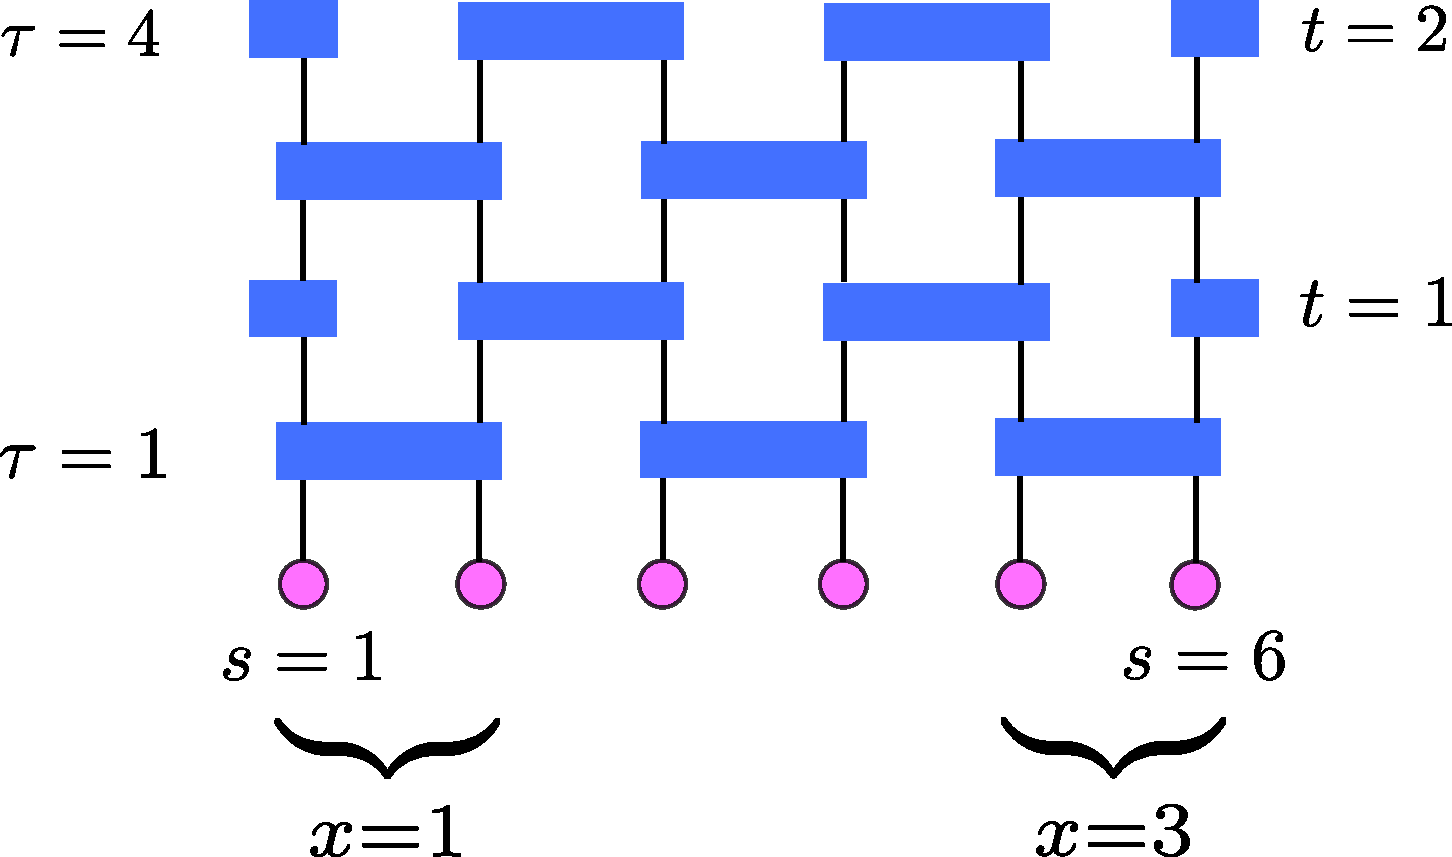
\includegraphics[width=.5\textwidth]{vonKgates}
	\caption{Brickwork architecture. In this figure $s$ and $\tau$ are the microscopic variables while $x$ and $t$ are the coarse-grained variables. Figure from~\cite{vonKeyserlingkHydro}.}
	\label{fig:vonKgates}
\end{figure}
The even-odd nature of the gates suggests defining two sets of variables: $(i,\t)$ increase by 1 at each site and after each layer of the circuit. On the other hand, $(x,t) = (i/2,\t/2)$ are defined so that all sites at integer $x$ are equivalent. The term ``coarse-graining" refers to the process of replacing $(i,\t)$ with $(x,t)$, but also refers to replacing these with continuous variables.

The ``random" part of random unitary circuits come from the choice of gates at each site. Each gate will be chosen from the Haar measure, a measure that is invariant under translations of the group manifold of gates. Essentially this just means a uniform distribution. If the circuit is unconstrained, the Haar measure is over all gates. If we want to include some conservation law, we divide the space of gates into sectors based on the conserved quantity and choose Haar-random gates within each sector. Sec.~\ref{sub:ccons} describes this process in detail.

\subsection{Floquet systems} \label{sub:floq}

In the next section we will discuss systems with no conservation laws. It would be nice to define the systems by their Hamiltonians, but any system with a Hamiltonian conserves energy. As discussed above, random circuits need not have any conserved quantities at all. How then can we compare them to any sort of Hamiltonian system?

The resolution lies in Floquet systems. In this branch of systems, there is a succession of Hamiltonians applied, each for a set amount of time. For example, if we ``turn on" Hamiltonian $H_1$ for time $T/2$ and then $H_2$ for $T/2$, then the Floquet unitary time evolution operator for one whole period of time $T$ is 
\begin{align}
U_F(T) = U_2\left(\frac{T}{2}\right)\; U_1\left(\frac{T}{2}\right) = e^{-i\frac{T}{2}H_2} e^{-i\frac{T}{2}H_1}.
\end{align}
For $t=nT$ with $n\in \mathbb{Z}$, the time evolution operator is $U(t)=U^n(T),$ while for noninteger multiples of $T$ it is more complicated. Hamiltonian and Floquet system are collectively referred to as \emph{physical systems.}

One example is the kicked Ising model~\cite{vonKeyserlingkHydro}, with 
\begin{align}
H_1 &= \phantom{h}\sum_i\left(Z_iZ_{i+1}+gZ_i\right),\nn
H_2 &= h\sum_iX_i. \label{eqn:kicked}
\end{align}
Note that all terms acting at a given time commute with each other. Therefore this Floquet model can be written as a unitary circuit (not random) with 2-site gates. 

Another example, from Refs.~\cite{ZhangFloq, ChenOtoc}, has time evolution operator 
\begin{align}
U_F(T) = e^{-i\frac{T}{2}H_x}e^{-i\frac{T}{2}H_z}, \label{eqn:gamma}
\end{align}
with
\begin{align}
H_x &= \sum_i g\Gamma X_j,\nn
H_z &= \sum_i \left[Z_iZ_{i+1} + (h+g\sqrt{1-\Gamma^2}G_i)Z_i\right],
\end{align}
where $G_i$ are independent Gaussian random variables. We will use the parameters $(g,h,T) = (0.9045,0.8090,0.8)$ throughout.
Note that as $\Gamma\to1$ this approaches the kicked Ising model, which thermalizes. As $\Gamma\to1$, this model becomes equivalent to the time-independent Hamiltonian $H=\sum_i\left[Z_iZ_{i+1} + h_iZ_i\right]$ with random field $h_i$, which is localized. For lack of a better term we will call Eq.~\ref{eqn:gamma} the $\Gamma$ model.

As in the previous section, we can study the transition between the localized and thermalizing phases by varying a parameter of the model, in this case $\Gamma$. Fig.~\ref{fig:floqtrans} demonstrates the transition using two diagnostics. 
\begin{figure}
	\centering
	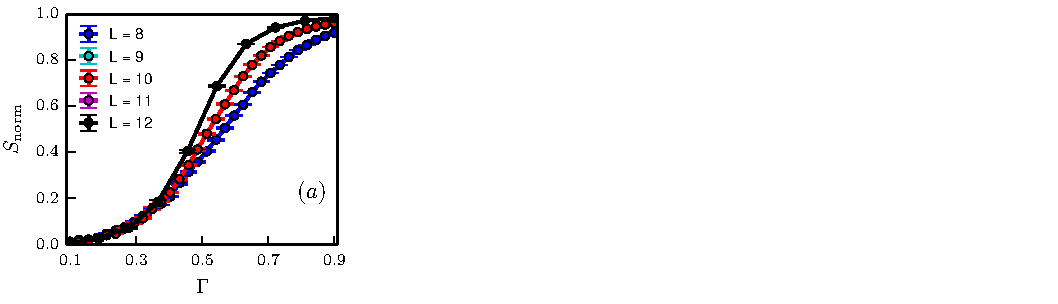
\includegraphics[width=.3\linewidth]{ZhangTransition1}
	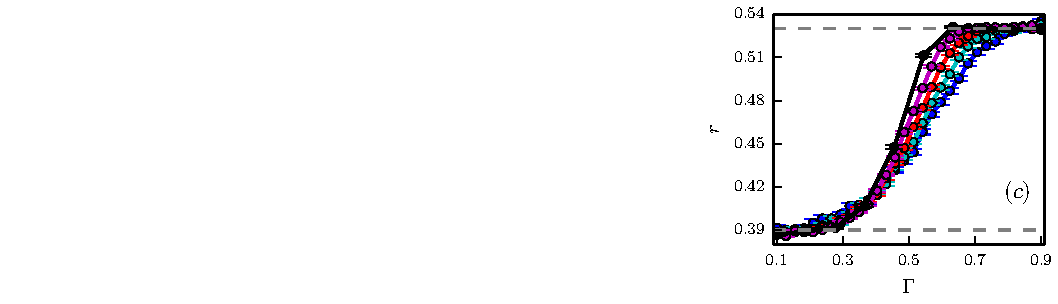
\includegraphics[width=.3\linewidth]{ZhangTransition2}
	\caption{Dynamical phase transition of the $\Gamma$ model. (a) demonstrates the phase transition through the average entanglement entropy between halves of the chain. (c) shows the same transition, but using the level statistics parameter. Figure from~\cite{ZhangFloq}.}
	\label{fig:floqtrans}
\end{figure}
The first is the entanglement entropy between two halves of the chain in energy eigenstates, 
\begin{align}
S_E \equiv -\Tr\{\rho_L\log\rho_L\} = -\Tr\{\rho_R\log\rho_R\},\label{eqn:Shalf}
\end{align}
where $\rho_L$ and $\rho_R$ are reduced density matrices of the right and left halves of the chain, with no relation to the operator right- and left-weights. The second equality in~\ref{eqn:Shalf} is due to the whole chain being in a pure state. The maximal possible entanglement between these halves is $S_\text{max}=L/2$, but random pure states will be close to the Page value~\cite{Page, ZhangTherm}
\begin{align}
S_R = \frac{L}{2} - \th{2\ln 2} -\mathcal{O}\left(\th{2^L}\right).
\end{align}

In the thermalizing phase the eigenstates have ``volume law" entanglement, close to $S_R$, while in the localized phase they have ``boundary law" entanglement, constant in $L$~\cite{ZhangFloq}. Therefore for large enough $L$, $S_E/S_R$ should distinguish between the phases. After averaging over all eigenstates for a given disorder realization and then averaging over disorder realizations, we arrive at $S_\text{norm} = \ex{S_E}/S_R$.

Alternatively we can use the level statistics parameter $r$ discussed previously. In the thermalizing phase the energies should be distributed according to the circular orthogonal ensemble with $r \approx 0.53$, while in the localizing phase the energies follow Poisson level statistics with $r\approx 0.39$. The dashed lines in Fig.~\ref{fig:floqtrans} show these values.

In Fig.~\ref{fig:floqtrans}, notice the agreement between the two diagnostics in the critical value $\Gamma_c$. Furthermore, both transitions become sharper for increasing $L$, as one would expect. The suggestion is that the transition is singular in the thermodynamic limit. In Sec.~\ref{sub:fncons} we will study this model at $\Gamma=.85$, deep in the thermalizing phase.


\section{Thermalization in systems with no conservation laws} \label{sec:ncons}

This section contains the phenomenology and analysis of thermalization of 

\subsection{Physical systems with no conservation laws} \label{sub:fncons}

As shown previously, the $\Gamma$ model with $\Gamma=0.85$ is deep within the thermalizing phase. Ref.~\cite{ChenOtoc} studied the OTO correlator of an initially local operator in this model. Recall that whereas thermalization is associated with a growing OTOC, it is associated with a decaying OTO correlator.

The key point is the exponential dependence of the OTO correlator. 
\begin{figure}
	\centering
	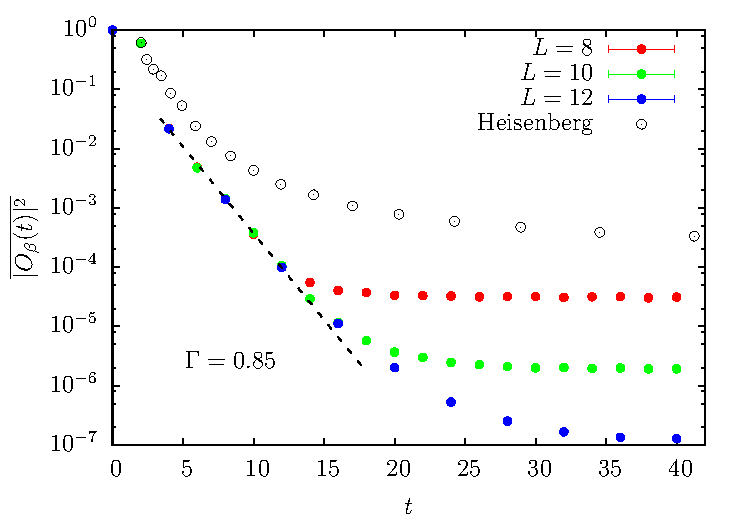
\includegraphics[width=.5\textwidth]{ChenExp}
	\caption{Exponential decay of the OTO correlator in a thermalizing Floquet model with no conserved charges~\cite{ChenOtoc}. For increasing system size, the decay continues to be exponential for a longer time before saturating. The black circles show the non-exponential decay of a Hamiltonian system. This decay is power-law, and will be discussed in the following section.}
	\label{fig:ChenExp}
\end{figure}
Fig.~\ref{fig:ChenExp} shows the exponential decay of the OTO correlator for various system sizes. Finite size effects cause the OTO correlator to saturate and therefore deviate from exponential behavior. However, the figure shows that this happens later for larger $L$, suggesting that the exponential decay continues for an arbitrarily long time for large enough $L$.

Ref.~\cite{vonKeyserlingkHydro} cranks $\Gamma$ all the way to 1, to study the kicked Ising model, defined in Eq.~\ref{eqn:kicked}. It goes beyond the early-time exponential dependence to study the saturation. The quantity under inspection is now the OTOC rather than the OTO correlator, so it should start at 0 and saturate to 1. There is also a focus on the operator right- and left-weights, $\rho_L$ and $\rho_R$.

Fig.~\ref{fig:vonKSpreading} shows the relevant quantities. Although it is for the quantum circuit, the qualitative behavior is the same (that's the whole point of this essay). At each site, exponential growth of both $\rho_R$ and the OTOC begins when the site enters the light cone. Exponential growth continues until the front reaches the site, at which point $\rho_R$ peaks and the OTOC begins to saturate. This front is the focus of Ref.~\cite{vonKeyserlingkHydro}.
Figs.~\ref{fig:vonKSpreading}~(a) and (b) can be thought of as horizontal slices though Fig.~\ref{fig:vonKSpreading}~(c). To compare with Fig.~\ref{fig:ChenExp}, imagine a vertical slice through~\ref{fig:vonKSpreading}~(c), with $t=0$ occurring at the position of the light cone.

The results, found through numerical simulation, are that the front propogates linearly at a velocity called the butterfly velocity, $v_B$. Consider $\rho(i,t)$. For $t<<v_B i$, the spreading operator has not yet reached $i$ and $\rho(i,t)$ is small. As the peak passes site $i$, a significant number of Pauli strings in the operator end on $i$. In the future, most strings end after $i$ so $\rho_R(i)$ is again small. For a given $t$, $\rho_R(i)$ peaks at $i=v_B t$. This peak has width $\sim t^\alpha$~\cite{vonKeyserlingkHydro}.
\begin{figure}
	\centering
	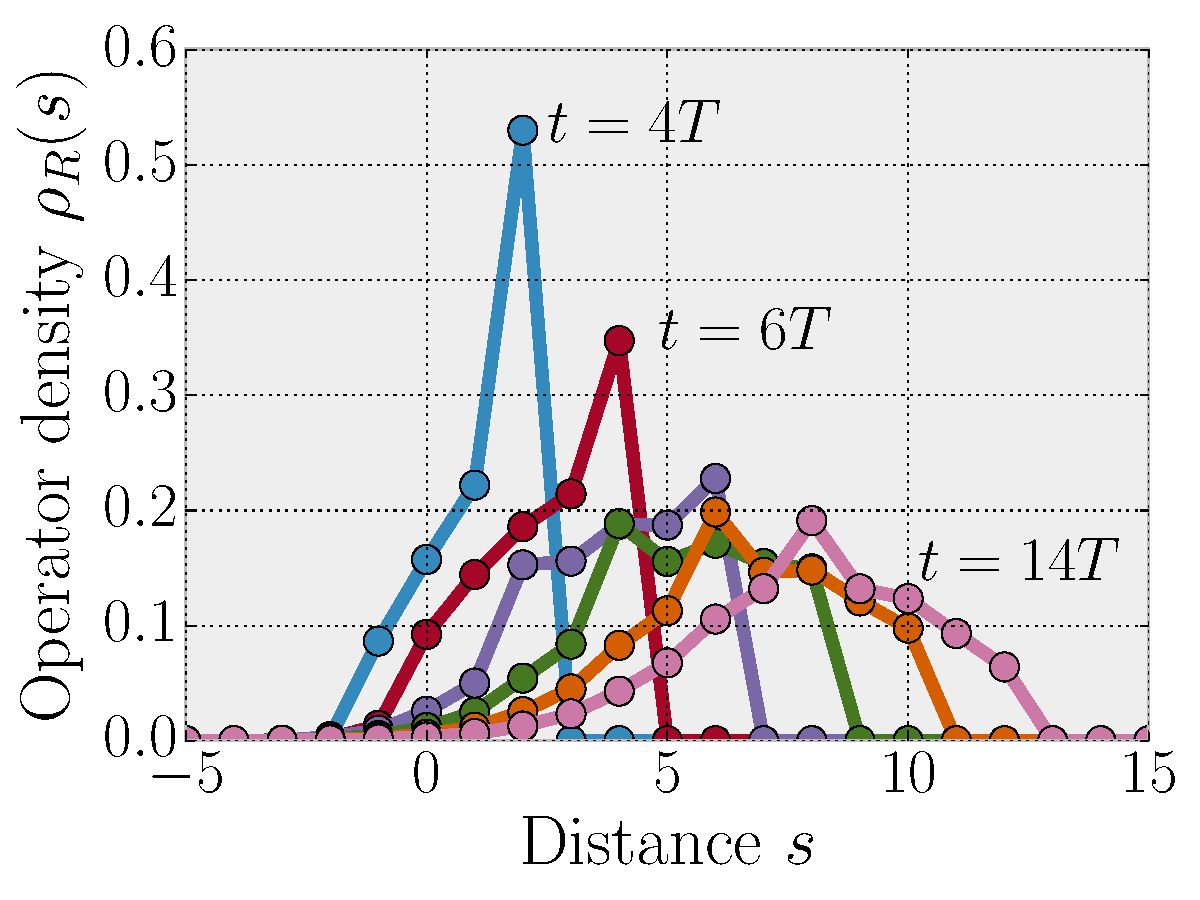
\includegraphics[width=.3\textwidth]{vonKpeaks}
	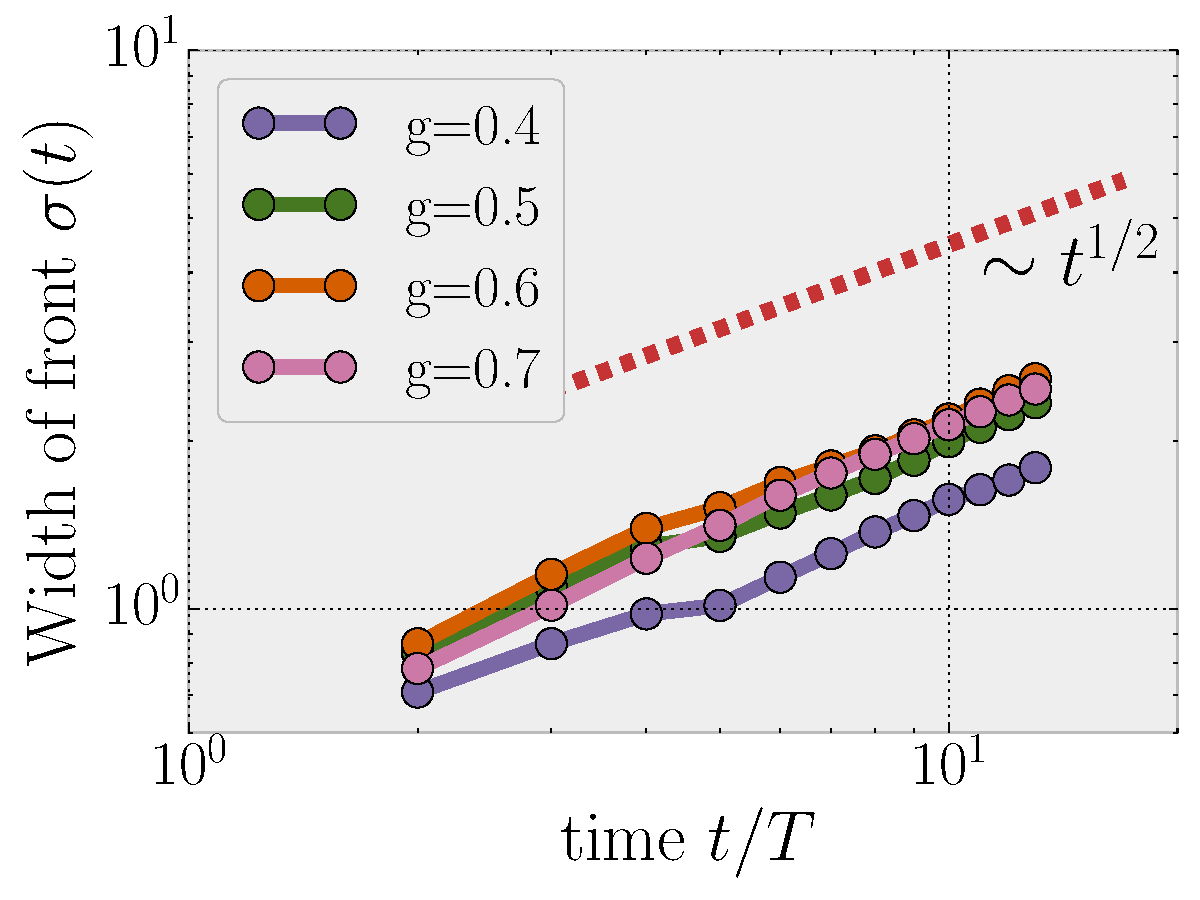
\includegraphics[width=.3\textwidth]{vonKalpha}
	\caption{Spreading of peaks in the kicked Ising model~\cite{vonKeyserlingkHydro}.}
	\label{fig:vonKalpha}
\end{figure}
Fig.~\ref{fig:vonKalpha} shows that $\alpha\approx .5$, so that the peaks spread with $\sqrt{t}$. This will be another test of our quantum circuits.

\subsection{Circuits with no conservation laws} \label{sub:cncons}

Early exponential growth.
Presence of front.
Broadening of front and exponential dependence therein.

The circuit under investigation in this section has the same architecture as Fig.~\ref{fig:circuit}, with each gate chosen from the Haar measure. Our goal is to find the dynamics of $\rho_R$ under the action of the full circuit, and our analysis will follow~\cite{vonKeyserlingkHydro}. The first step in doing so is to calculate the dynamics of $\rho_R$ under a single gate. 

We want to calculate $\rho_R(i,\tau+1)$ and $\rho_R(i+1, \tau+1)$ (Fig.~\ref{fig:2sites}). It should be clear that these quantities only depend on $\rho_R(i,\tau)$ and $\rho_R(i+1, \tau)$. In fact it is even simpler, in that $\rho_R(i,\tau+1)$ and $\rho_R(i+1, \tau+1)$ only depend on the sum $\rho_R(i,\tau) + \rho_R(i+1, \tau)$. 

\begin{figure}
	\centering
	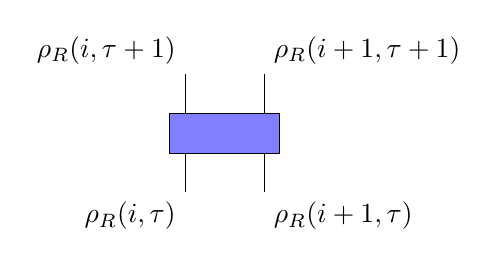
\begin{tikzpicture}[scale = 1]
\draw (0,0) node[below left]{$\rho_R(i,\tau)$} -- (0,1.5) 
			node[above left]{$\rho_R(i,\tau+1)$};
\draw (1,0) node[below right]{$\rho_R(i+1,\tau)$} -- (1,1.5)
			node[above right]{$\rho_R(i+1,\tau+1)$};

\filldraw[color=black, fill=blue!50] (-.2,.5) rectangle (1.2,1);


\end{tikzpicture}
	\caption{Diagram of the operator weights before and after the application of the gate. Values at $\t+1$ are calculated in the text.}
	\label{fig:2sites}
\end{figure}

Looking at $\rho_R(i,\tau)$ and $\rho_R(i+1, \tau)$ is equivalent to looking only at Pauli strings which are $I$ on all sites past $i+1$ but are non-identity on either $i$ or $i+1$ (or both).
This leaves us with $q^4-1$ two-site operators to consider. The Haar-random gate transforms any of these operators to any other with equal probability~\cite{BrownScrambling}, regardless of whether the initial operator was an identity on site $i+1$. This is why the final values only depend on $\rho_R(i,\tau) + \rho_R(i+1, \tau)$.

Of the $q^4+1$ final operators, $q^2-1$ are the identity on site $i+1$. These operators contribute to $\rho_R(i,\tau+1)$, while the rest contribute to $\rho_R(i+1, \tau+1)$. In other words the weight moves to site $i$ with probability $p_\text{back} = \frac{q^2-1}{q^4-1} = \th{q^2+1}$ or moves forward with probability $p\equiv 1- p_\text{back} = \frac{q^2}{q^2+1}$. Thus
\begin{align}
\rho(i,\t+1) &= (1-p)\left[\rho(i,\t)+\rho(i+1,\t)\right],\nn
\rho(i+1,\t+1) &= p\left[\rho(i,\t)+\rho(i+1,\t)\right].
\end{align}
This is true at each individual gate. If there were a gate at each site at each time, this would be the final word. However, since the dynamics will only be periodic in every two layers of the circuit, we must calculate the dynamics for two layers to get the whole picture.

To do so, we will define some dense but useful notation. Since the sum of weights at consecutive sites is so important, we will abbreviate it as
\begin{align}
\tilde{\rho}_R(i,\t) \equiv \rho_R(i,\tau) + \rho_R(i+1, \tau). \label{eqn:rhotil}
\end{align}
We will want to find $\tilde{\rho}_R(i,\t+2)$. To do so we find
\begin{align}
\rho_R(i-1, \t+1) &=    p  \tilde{\rho}_R(i-2, \t),\nn
\rho_R(i  , \t+1) &= (1-p) \tilde{\rho}_R(i  , \t),\nn
\rho_R(i+1, \t+1) &=    p  \tilde{\rho}_R(i  , \t),\nn
\rho_R(i+2, \t+1) &= (1-p) \tilde{\rho}_R(i+2, \t).\label{eqn:4sites1}
\end{align}
Similar calculation at time $\t+2$ result in
\begin{align}
\rho_R(i  , \t+2) &= p^2\tilde{\rho}_R(1-2,\t) + p(1-p)\tilde{\rho}_R(i,\t),\nn
\rho_R(i+1, \t+2) &= p(1-p)\tilde{\rho}_R(i,\t) + (1-p)^2\tilde{\rho}_R(i+2,
	\t), \nn
\tilde{\rho}_R(i,\t+1)&=p^2\tilde{\rho}_R(i-2,\t)+2p(1-p)\tilde{\rho}_R(i,\t)+
	(1-p)^2\tilde{\rho}_R(i+2,\t). \label{eqn:4sites2}
\end{align}
Fig.~\ref{fig:4sites} shows a diagram containing these values.
\begin{figure}
	\centering
	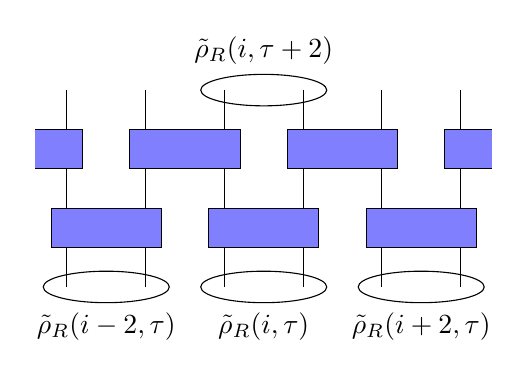
\begin{tikzpicture}[scale = 1]
\draw (0,0) -- (0,2.5);
\draw (1,0) -- (1,2.5);
\draw (2,0) -- (2,2.5);
\draw (3,0) -- (3,2.5);
\draw (4,0) -- (4,2.5);
\draw (5,0) -- (5,2.5);

\foreach \x/\y in {0/1, 2/1, 4/1, 1/2, 3/2} 
\filldraw[color=black, fill=blue!50] (\x-.2,\y-.5) rectangle (\x+1.2,\y);

\draw (0.5,0) circle [x radius=.8, y radius=.2];
\draw (0.5,-0.2) node[below]{$\tilde{\rho}_R(i-2,\t)$};
\draw (2.5,0) circle [x radius=.8, y radius=.2];
\draw (2.5,-0.2) node[below]{$\tilde{\rho}_R(i,\t)$};
\draw (2.5,2.5) circle [x radius=.8, y radius=.2];
\draw (2.5,2.7) node[above]{$\tilde{\rho}_R(i,\t+2)$};
\draw (4.5,0) circle [x radius=.8, y radius=.2];
\draw (4.5,-0.2) node[below]{$\tilde{\rho}_R(i+2,\t)$};

\draw[fill=blue!50] (-.4,1.5) -- (.2,1.5) -- (.2,2) -- (-.4,2);
\draw[fill=blue!50] (5.4,2) -- (4.8,2) -- (4.8,1.5) -- (5.4,1.5);

\end{tikzpicture}
	\caption{Operator weights after two layers of the circuit}
	\label{fig:4sites}
\end{figure}

The fact that $i\pm1$ and $\t\pm1$ do not appear in Eq.~\ref{eqn:4sites2} demonstrates the usefulness of the coarse-grained variables, defined in Fig.~\ref{fig:circuit}. Switching to those variable and dropping the tilde, Eq~\ref{eqn:4sites2} becomes
\begin{align}
\rho_R(x,t+1)&=p^2\rho_R(x-1,t)+2p(1-p)\rho_R(x,t)+(1-p)^2\rho_R(x+1,t), 
	\label{eqn:4sites3}
\end{align}
which is the equation for a biased random walk that steps to the right with probability $p^2$ and to the left with probability $(1-p)^2$, otherwise staying at the same site. 

Therefore, for any operator initially local at position $x_0$, $\rho_R$ spreads linearly with a front located near position $x = x_0 + v_B t$. The front spreads diffusively as $\ex{x^2}-\ex{x}^2=2Dt$~\cite{vonKeyserlingkHydro}. The values are
\begin{align}
v_B &= p^2-(1-p)^2 = \frac{q^2-1}{q^2+1},\nn
D   &= \sqrt{1-v_B^2}/4 = \frac{q/2}{q^2+1}.
\end{align}
These results can be summarized in Fig.~\ref{fig:vonKSpreading}.
\begin{figure}
	\centering
	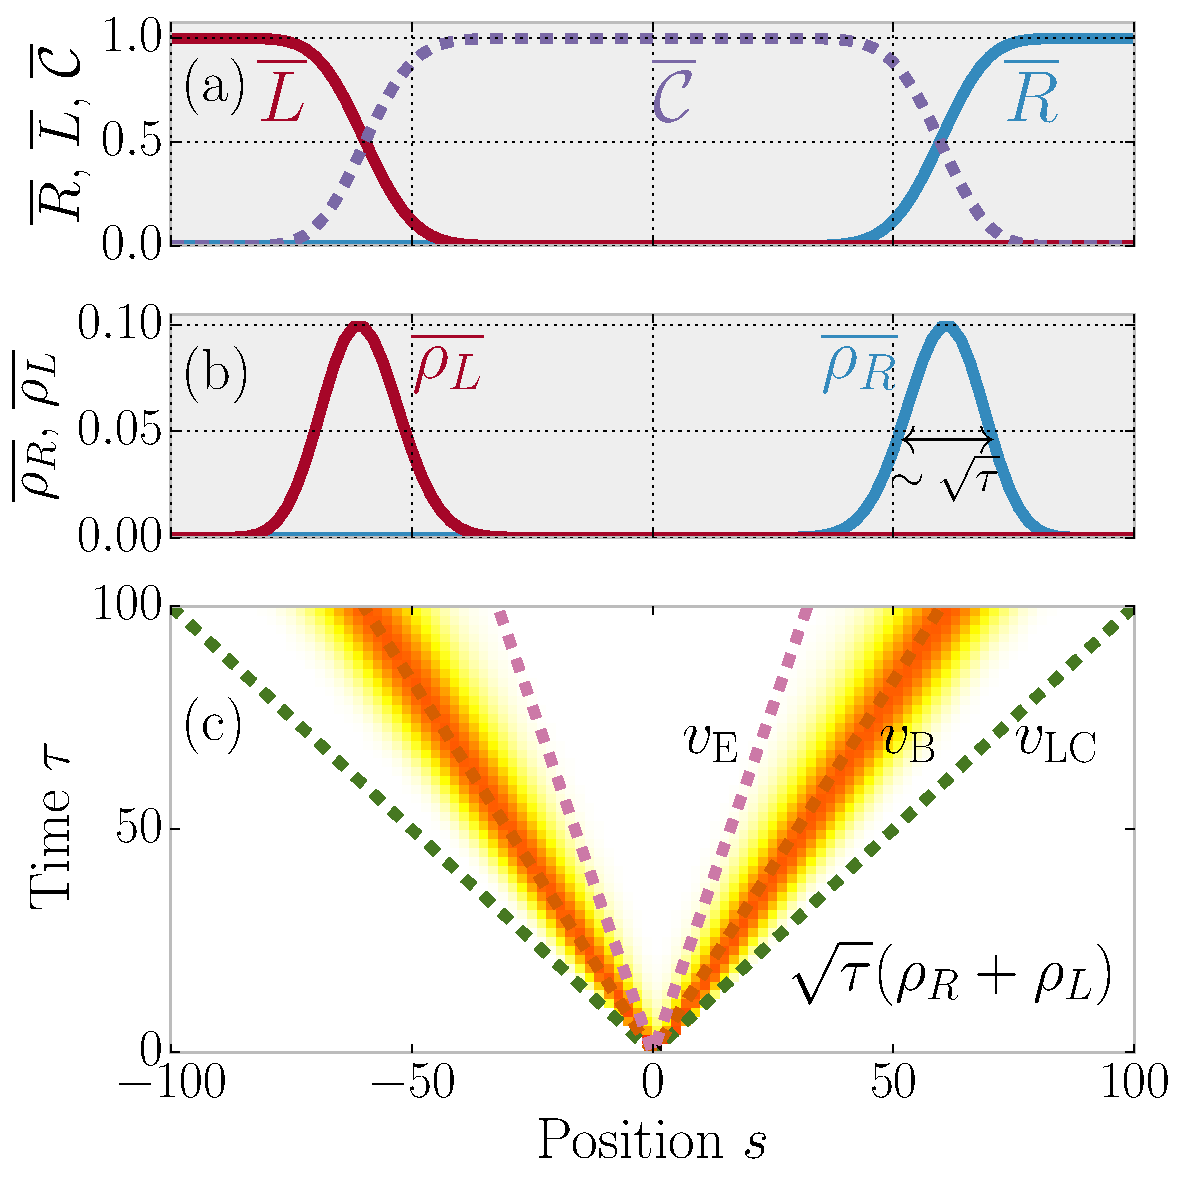
\includegraphics[width=.5\textwidth]{vonKSpreading}
	\caption{Spreading of an initially local operator under a quantum circuit with no conservation laws~\cite{vonKeyserlingkHydro}.}
	\label{fig:vonKSpreading}
\end{figure}
As an interesting aside, note that in the large $q$ limit the front does not diffuse and $v_B=1$, the lightcone velocity~\cite{NahumOpSp}.

The important features that we can match to the behavior of the floquet model are the exponential growth at early time and the behavior of the front of the spreading operator. As in the kicked Ising model, we have shown that the front moves linearly. The diffusion process has a width $\sim \sqrt{Dt}$, which is to say $\alpha=0.5$

\note{vonKeyserlingk page 6.}


\section{Thermalization in systems with conservation laws} \label{sec:cons}

Introducing conserved charges to our systems slows down their dynamics. In this section we will see how this process occurs, in both physical systems and quantum circuits. It is straightforward to introduce conserved charges to the circuits by restricting to gates that satisfy some conservation law. For the physical systems we have two ways to proceed. We can either consider Floquet systems with conservation laws, or systems with time-independent Hamiltonians (with or without further conservation laws).

\subsection{Floquet systems with conserved quantities} \label{sub:fcons}

We can introduce conserved charges to Floquet systems by ensuring that both partial Hamiltonians in the model obey some conservation law. Ref.~\cite{KhemaniOpSp} studies a model with time evolution operator
\begin{align}
U_F(T)=e^{i\frac{T}{2}H_z}e^{i\frac{T}{2}H_{xy}},
\end{align}
where
\begin{align}
H_z &= J_z\sum_i Z_iZ_{i+1},\nn
H_{xy} &= J_{xy}\sum_i\left[X_iX_{i+1}+Y_iY_{i+1}\right].
\end{align}

\note{In these ``physical systems," it is possible to have approximately conserved charges, i.e. on the localized side of a phase transition\dots}

\subsection{Constrained circuits and conserved operators} \label{sub:ccons}

A simple conservation law to introduce to quantum circuits is conservation of total $Z$. We simply have to constrain the 2-site gates to conserve $Z_\tot$ for the two sites on which it acts. $Z_\tot$ is then our conserved charge, with charge density $Z_i$.
We will use spin-$\th{2}$ sites, so gates will be in the $\uparrow\uparrow\to\uparrow\uparrow$, $\downarrow\downarrow\to\downarrow\downarrow$, or $\{\uparrow\downarrow,\downarrow\uparrow\}\to\{\uparrow\downarrow,\downarrow\uparrow\}$ sectors. We will refer to these as the $Z=1$, $Z=0$, and $Z=-1$ sectors, of dimension 1, 4, and 1, respectively. The matrix representations of gates will be $4\times4$ matrices made up of three block matrices, one for each sector.

Like in the unconstrained circuit, we want to have an on-site dimension $q$ that we can use to vary the behavior of the circuit. It would also be nice to preserve the block structure of the gates as we vary $q$, which would not be possible if we replace the spin-$\th{2}$ sites with higher spin. We can satisfy both of these requests by instead replacing the spins with a tensor product between a spin-$\th{2}$ degree of freedom and an unconstrained $q$-dimensional qudit. We do not constrain the gates' action on the qudits.
This leaves us with $4q^2\times4q^2$ block-diagonal gates, with blocks of size $q^2\times q^2$, $2q^2\times 2q^2$, and $q^2\times q^2$ (Fig.~\ref{fig:khemaniCircuit}).

\begin{figure}
	\centering
	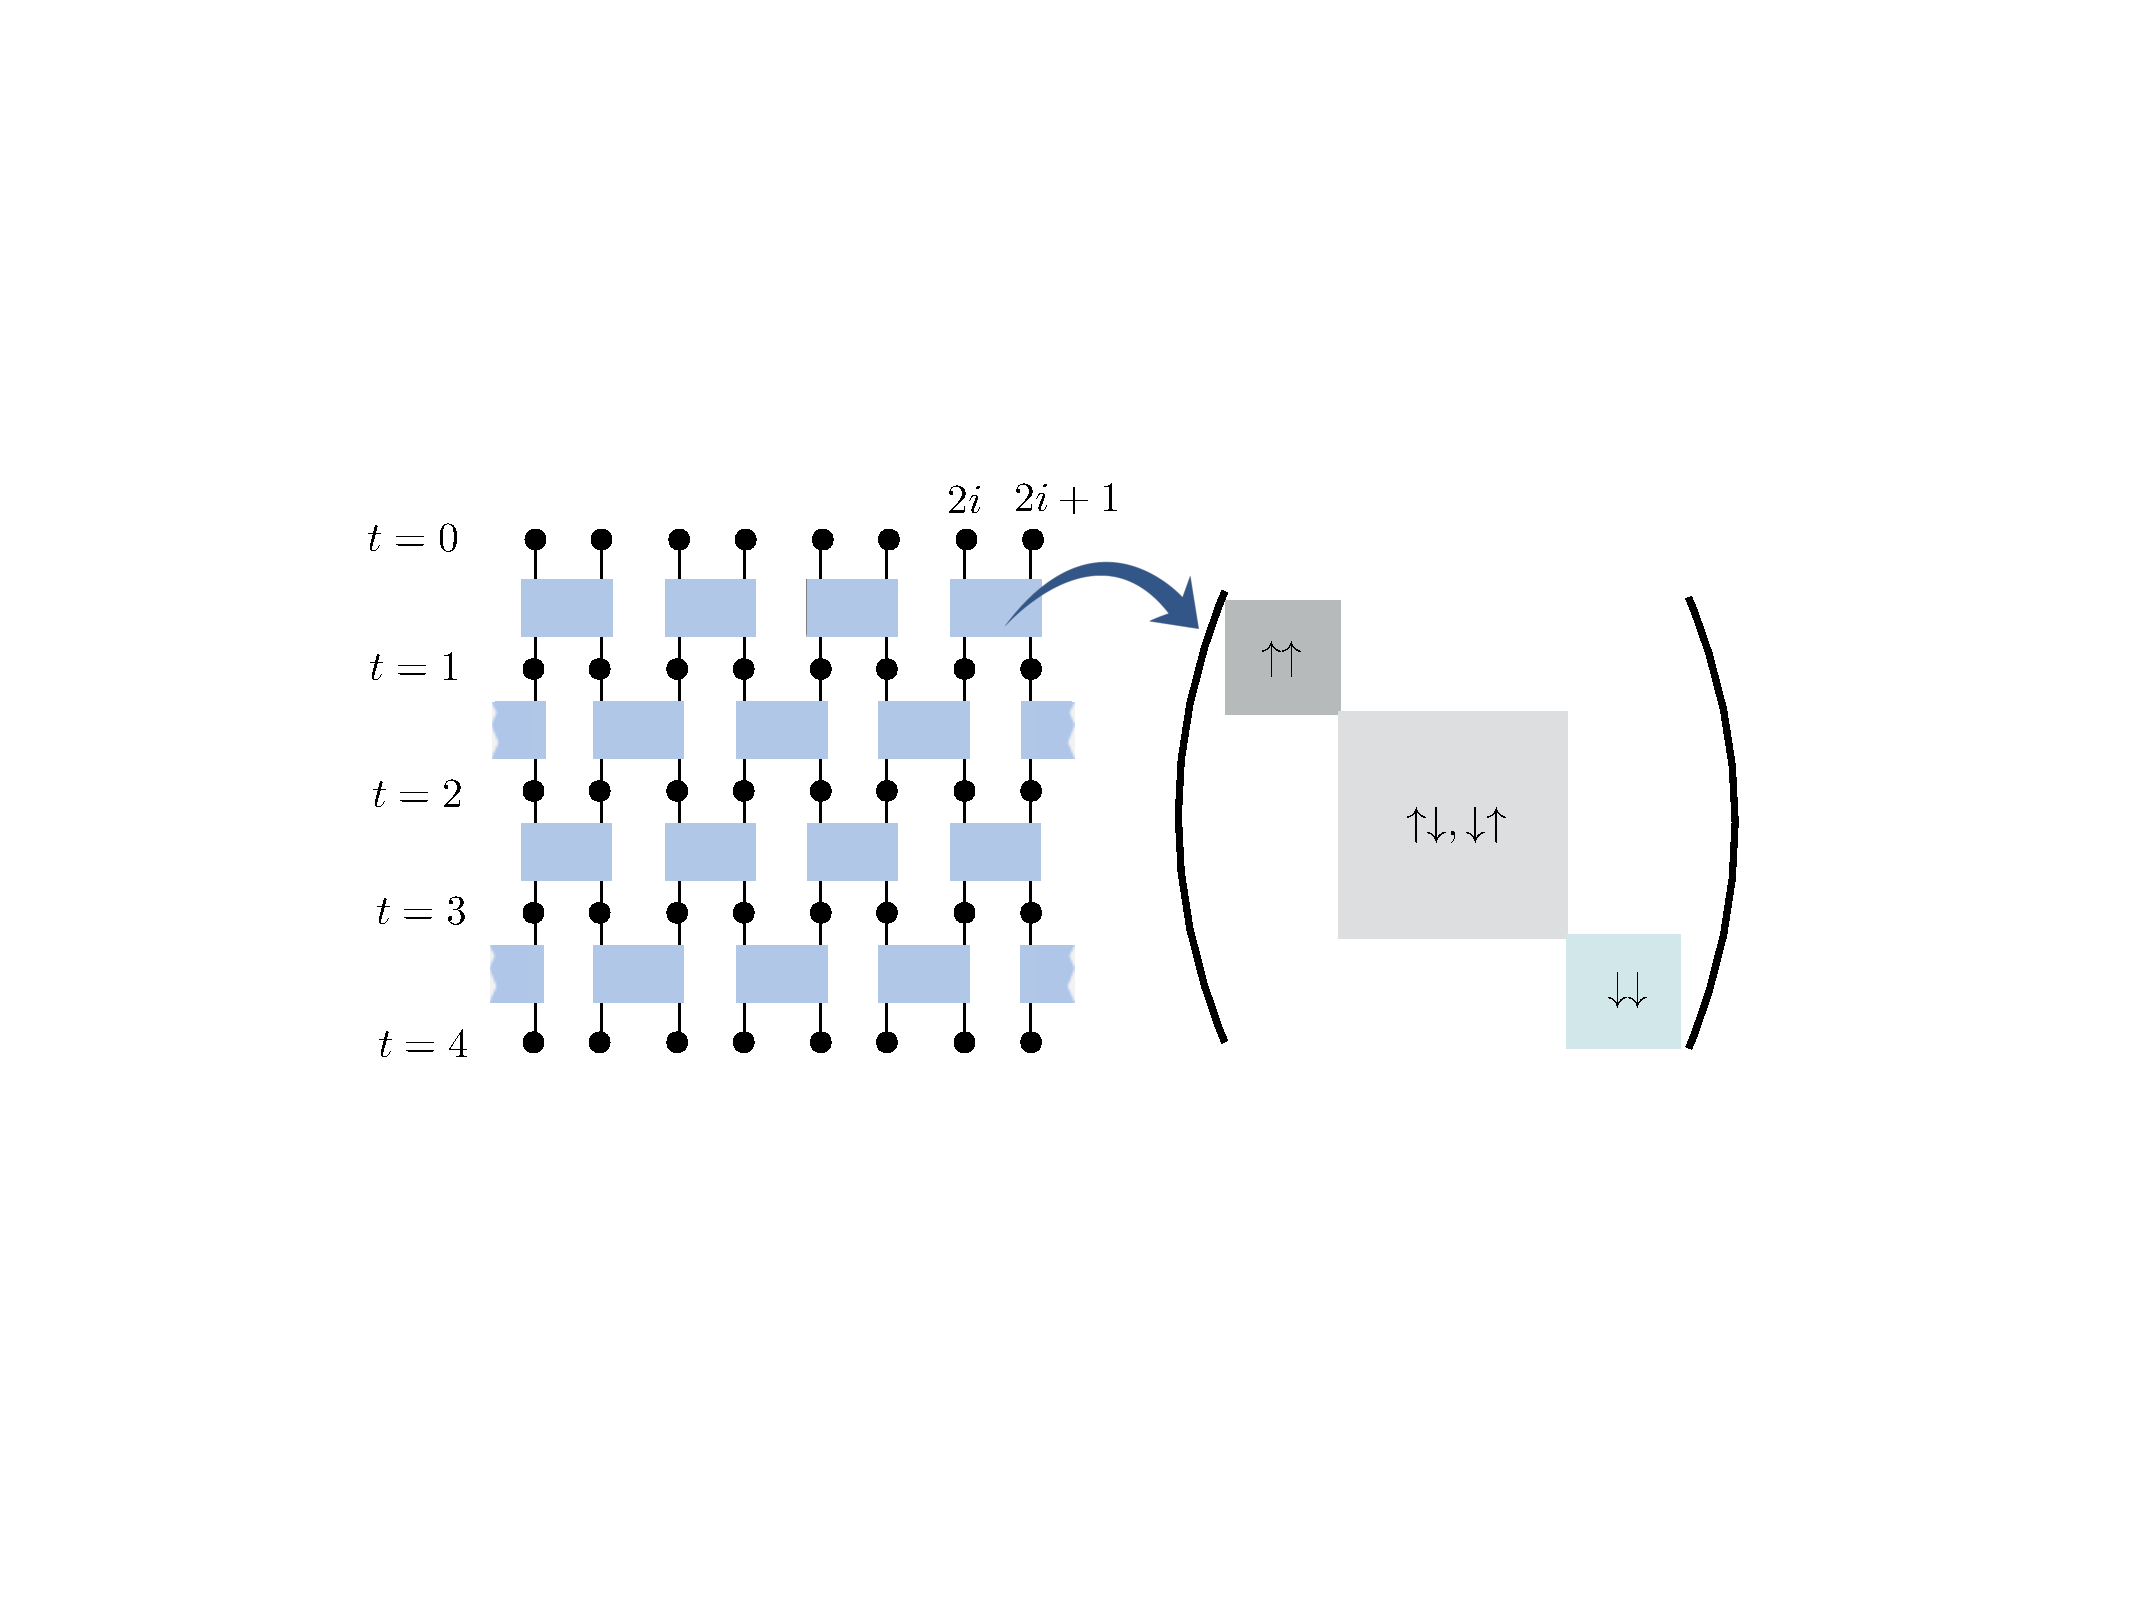
\includegraphics[width=.5\textwidth]{khemaniCircuit}
	\caption{A quantum circuit constrained to conserve $Z_\tot$. The three blocks are of dimension $q^2\times q^2$, $2q^2\times 2q^2$, and $q^2\times q^2$. Figure from~\cite{KhemaniOpSp}.}
	\label{fig:khemaniCircuit}
\end{figure}

The next step is to define a basis for our operators. On the qudit, we will continue to use an abstract Pauli basis $\Sigma_i^\nu$, $\nu=0,\dots,q^2-1$. On the qubit, instead of the usual Pauli operators, we will use the basis~\cite{KhemaniOpSp}
\begin{align}
\{\sigma_i^{\mu=0,1,2,3}\} \equiv \{I_i, R_i, L_i,Z_i\}=\{I_i,\frac{\sigma_i^+}{\sqrt{2}}, \frac{\sigma_i^-}{\sqrt{2}}, \sigma_i^z\}
\end{align}
We have chosen $\sigma_i^1, \sigma_i^2$ to be normalized raising/lowering operators, or equivalently charge creation/annihilation operators. Then the basis on site $i$ is $B_i^{\mu\nu} \equiv \sigma_i^\mu \otimes \Sigma_i^\nu$. We will write these as $(I\Sigma^\nu)_i$, $(Z\Sigma^\nu)_i$, etc. The basis strings will be of the form \note{$\S=\otimes_iB_i^{\mu_i\nu_i}$.}

Some operators are special because they measure the conserved charge. The local charge density is $Z_i=(ZI)_i$, while the total charge is $Z_\tot=\sum_i(ZI)_i$. Charge conservation is written as 
\begin{align}
Z_\tot(t) = U(t)^\dag Z_\tot(0)U(t) = Z_\tot(0), \label{eqn:cons}
\end{align}
where $U(t)$ is the combined action of the entire circuit.

Along the way to defining the right-weight, we defined the operator amplitude
\begin{align}
a_\S(t) = \th{q^L}\Tr\{ \cal{O}(t)\S \},\quad \sum_S\abs{a_\S} = 1, \label{eqn:unit}
\end{align}
with the latter equality imposed by unitarity. For the new conserved charge we can define the conserved operator amplitude,
\begin{align}
a_i^c(t) = \th{(2q)^{L}}\Tr\{\cal{O}(t)(ZI)_i\},
\end{align}
and  the ``conserved part" of $\cal{O}(t)$,
\begin{align}
\cal{O}^c(t)=\sum_i a_i(t)(ZI)_i.
\end{align}
The conservation law~(\ref{eqn:cons}) is then equivalent to 
\begin{align}
\sum_i a_i^c(t)=\sum_i a_i^c(0). \label{eqn:consa}
\end{align}
Note that Eq.~\ref{eqn:consa} refers to amplitudes, while Eq.~\ref{eqn:unit} refers to squares of amplitudes. Later, we will also want to refer to the conserved and nonconserved right-weights, 
\begin{align}
\rho^c(i,t) = \abs{a^c_i(t)^2}, \quad \rho_R^\nc(i,t) = \rho_R(i,t)- 
	\rho^c(i,t).
\end{align}

\subsection{Operator spreading in conserving circuits} \label{sub:consop}

We are now ready to discuss the spreading of operators. We will consider the operator $(ZI)_0$ where $i=0$ is the middle of a long chain. There will be three behaviors extracted from our model: diffusion of the conserved operators (forming a ``lump"), ballistic propagation of the ``front" of nonconserved operators, and a power-law ``tail" of nonconserved operators behind the front. Fig.~\ref{fig:khemaniRWeight} illustrates these three regimes.

We'll start with the conserved operators. The effect of a Haar-random unitary acting on sites $i$ and $i+1$ is to average the conserved amplitudes, so that
\begin{align}
a^c_i(t+1)=a^c_{i+1}(t+1) = \frac{a^c_i(t)+a^c_{i+1}(t)}{2}, \label{eqn:ampevol}
\end{align}
where equality holds after Haar-averaging.\footnote{We will we be cavalier about our Haar-averaging. For exact statements see Ref.~\cite{KhemaniOpSp}.} After coarse graining $i\to x$, in the $x, \to\infty$ limit, this behavior results in 
\begin{align}
a^c(x,t) = \sqrt{\frac{1}{2\pi t}}e^{-\frac{x^2}{2t}},
\end{align}
which is a diffusing lump with diffusion constant $D_c=\th{2}$. Therefore the total weight on conserved operators falls over time,
\begin{align}
\rho^c_\tot(t) \simeq \int dx\,\abs{a^c(x,t)} = \int dx\,\th{2\pi t}e^{-x^2/t} 
	=\th{2\sqrt{\pi t}}, \label{eqn:rhoc}
\end{align}
with power-law dependence.

If $\rho^c$ is decreasing, then $\rho^\nc$ must be increasing. The effect of Eq.~\ref{eqn:ampevol} is to decrease $\rho^c(i,t)$ by
\begin{align}
\delta \rho^c_i(t) = -\frac{(a^c_i(t)-a^c_{i+1}(t))^2}{2}.
\end{align}
All of this weight gets shuffled into nonconserved operators. But we know how nonconserved operators spread! In fact, we can simply use the analysis of the previous section to say that there is a front that travels at $v_B$, broadening diffusively with width $\sim\sqrt{D_\rho t}\sim\sqrt{t/q^2}$. In the large $q$ limit, the diffusivity vanishes and therefore the front has zero width.

If there were no remaining lump at the origin, our description of the front would be complete. However, even at late time the lump of conserved operators is emitting nonconerved operators. These operators form a tail lagging behind the front. Since the lump shrinks as a power law in time and all nonconserved operators travel at $\sim v_B$, the tail has a power-law shape in space. In fact, at time $t$ and position $x$, with $x$ well separated from the origin and from $v_Bt$, the majority of $\rho^\nc_R(x,t)$ comes from operators emitted from the lump at time $t-x/v_B$. If the lump is far away, it can be approximated by a point source with all weight at the origin, emitting nonconserved operators proportional to the decrease in $\rho^c_\tot$. So,
\begin{align}
\rho_R^\nc(x,t)\sim\pd{\rho_\tot^c(t-x/v_B)}{t} \sim\th{(t-x/v_B)^{3/2}}. 
	\label{eqn:powtail}
\end{align}
The fact that the spacial exponent $-3/2$ is equal to $-1/2-1$, where $-1/2$ is the time exponent of the decrease of $\rho_\tot^c$, will become important in our analysis of the fracton circuit.

Since this analysis became abstract rather quickly, Fig.~\ref{fig:khemaniRWeight} shows the qualitative pictures for operators spreading.
\begin{figure}
	\centering
	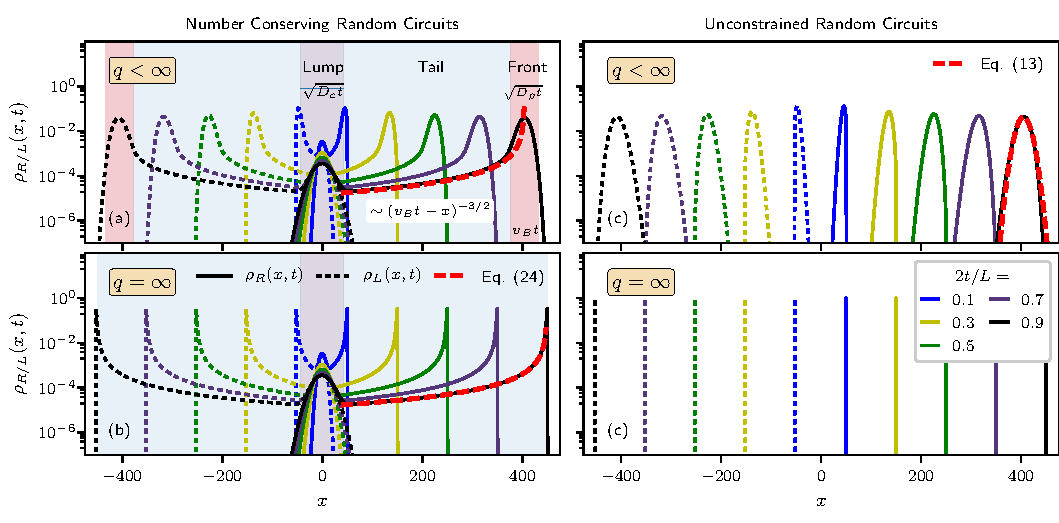
\includegraphics[width=\textwidth]{khemaniRWeight}
	\caption{Comparison of circuits with and without conservation laws, at finite and infinite $q$. Each solid line is a right-weight and each dashed line (except red) is a left-weight. (a): the vertical shading corresponds to the three parts of the operator at $2t/L=0.9$, the lump, the tail, and the front. The lump consists of conserved operators and broadens diffusively. The front consists of nonconserved operators emitted at early time and travels ballistically. The tail consists of nonconserved operators emitted at later time and has approximate power-law behavior $\sim(v_Bt-\abs{x})^{-3/2}$ (shown by the red dashed line). (b): In the large $q$ limit, the front has width $=0$ and does not broaden at all (just as in the nonconserving circuit). (c,d): In the nonconserving circuit there are no conserved operators and therefore no central lump. Since the power-law tail is emitted by the lump, there is no such tail in this case either. The only structure is broadening front. As discussed previously, the front does not broaden in the large $q$ limit. Figure from~\cite{KhemaniOpSp}.}
	\label{fig:khemaniRWeight}
\end{figure}
It includes the large $q$ (ideal) behavior for conserving and nonconserving circuits and also shows how finite $q$ affects these values. The first subfigure shows the lump, front, and tail, while some or all of those features are absent in other systems.

Now that we have fully described the operator spreading for conserving circuits, we are ready to explain the power-law dependence of the OTO correlator in Sec~\ref{sub:fcons}. We will use the language of the OTOC, though, because this is the quantity more commonly seen in the literature now.

Once the operator front is far past $x$ ($v_Bt>>\abs{x}+\sqrt{D_\rho t}$), most strings that have spread past $x$ look random, so they contribute to the equilibrium value of the OTOC,\footnote{This is a simplification. See~\cite{KhemaniOpSp} for details} which is 1. The deviation from the equilibrium value can only be due to operators that have not yet reached $x$ at time $t$, so they must have been at the origin at time $t'=t-x/v_B$. Since the only operators at the origin are the conserved operators, so using~(\ref{eqn:ampevol}) we have
\begin{align}
1-C(x,t) = \rho^c_\tot(t-x/v_B) = \th{2\sqrt{\pi(t-x/v_B)}}.
\end{align}
Since the OTOC and the OTO correlator are linearly related~(\ref{eqn:OTOCOTO}), this explains the power-law dependence in Sec~\ref{sub:fcons}.

The material so far has introduced all of the dynamics-based material we will need to understand fractonic circuits, but we haven't covered fractons yet! We'll take a brief tour into the physics of fractons before circling back to see how we can understand localization in fractonic circuits using our previous analysis of thermalizing circuits.


\section{Fractonic systems} \label{sec:frac}

In this section we will explore various fractonic systems. We will start with exactly solvable models and show that these naturally result in massive (gapped) fractons. However we will quickly transition to tensor gauge theory, where we can create gapless fractons. Ultimately, we want to show the connection between multipole conservation laws (specifically dipole) and fractons. This motivates the study of random circuits that conserve dipole moment as a setting for localized charges, which will be presented in Sec.~\ref{sec:fraccirc}.

The conservation of dipole moment means that an isolated charge cannot move without creating an isolated dipole somewhere else, which costs energy. Thus, the charges are immobile in the low-energy limit. 

\subsection{Tensor gauge theory} \label{sub:tensor}

We will show how fracton conservation laws naturally lead to tensor gauge theory. Although this is not strictly necessary to understand the dynamics of fracton systems, the literature often refers to fractons using the language of tensor gauge theory. This discussion follows the treatment in~\cite{PretkoFractonGauge}. 

To start, we will briefly review the familiar form of U(1) gauge theory. Consider a complex scalar field $\phi(x,t)$. We will treat time and space separately despite the theory being Lorentz invariant because the fracton theory is not Lorentz invariant. The charge density of this field is $\rho =\phi^\dag\phi$, with total charge $Q=\int d^dx \rho$. Requiring $Q=\text{const.}$ is equivalent to \note{requiring
\begin{align}
\phi\to e^{i\alpha}\phi
\end{align}	
be a symmetry of the theory,} for constant $\alpha$. At this point $\phi$ and all of its derivatives and powers transform covariantly, which is to say that each operator transforms as $\mathcal{O}\to e^{in\alpha}\mathcal{O}$ under the phase rotation.

Gauging this theory requires that the theory be invariant under $\phi\to e^{i\alpha(x,t)}\phi$ for arbitrary $\alpha(x,t)$. However, the derivative of the field now transforms as 
\begin{align}
\partial_i\phi\to e^{i\alpha}\left(\partial_i+\partial_i\alpha\right)\phi,\nn
\partial_t\phi\to e^{i\alpha}\left(\partial_t+\partial_t\alpha\right)\phi.
	\label{eqn:nconv}
\end{align}
This is not a covariant transformation, as it mixes the derivatives of $\phi$ with $\phi$ itself. The standard solution is to introduce gauge derivatives $D_i=\partial_i-iA_i$ and $D_t=\partial_t-i\Phi$, where $\Phi$ recalls the notation for the scalar potential of electromagnetism. We then have 
\begin{align}
D_i\phi\to e^{i\alpha}D_i\phi,\nn
D_t\phi\to e^{i\alpha}D_t\phi,
\end{align}
if 
\begin{align}
A_i &\to A_i+\partial_i\alpha, \nn
\Phi&\to\Phi+\partial_t\alpha.
\end{align}
We can then go on to calculate field strengths and possible terms in the action, but our main interest is in the fact that the gauge field is a spacetime vector $A_\mu=(\Phi,A_i)$. For more details see~\cite{PretkoFractonGauge}.

We will now go through the same steps for a fracton field $\phi$ in order to show the natural emergence of symmetric tensor gauge fields. $\phi$ is again a complex scalar that conserves charge $Q=\int d^dx\rho$. It also conserves dipole moment $P_i = \int d^dx\rho x^i$ (breaking Lorentz invariance). Together these correspond to phase rotations of the form 
\begin{align}
\phi\to e^{i\alpha+i\lambda_ix^i}\phi.
\end{align}
We will write this phase as $e^{i\alpha(x)}$ where $\alpha$ is restricted to be linear until we gauge the theory.

Now $\partial_i\phi\to e^{i\alpha}(\partial_i+\lambda_i)\phi$ is no longer covariant. The second derivative 
\begin{align}
\partial_i\partial_j\phi\to e^{i\alpha}(\partial_i\partial_j+\lambda_i\partial_j+\lambda_j\partial_i)\phi
\end{align}
looks slightly more promising because its symmetric structure can also be obtained from the operator $\partial_i\phi\partial_j\phi$. In fact, the lowest order operator is~\cite{PretkoFractonGauge}
\begin{align}
\phi\partial_i\partial_j\phi-\partial_i\phi\partial_j\phi \to e^{2i\alpha} \left(\phi\partial_i\partial_j\phi-\partial_i\phi\partial_j\phi\right).
\end{align}
This means that the action can contain this operator.

Gauging the fracton theory so that $\alpha$ is again an arbitrary function, we now find
\begin{align}
\phi\partial_i\partial_j\phi-\partial_i\phi\partial_j\phi \to e^{2i\alpha} \left(\phi\partial_i\partial_j\phi-\partial_i\phi\partial_j\phi + i(\partial_i\partial_j\alpha)\phi^2\right).
\end{align}
This suggests that, instead of constructing the covariant first derivative $D_i\phi$, we construct a covariant second derivative 
\begin{align}
D_{ij}\phi^2=\phi\partial_i\partial_j\phi-\partial_i\phi\partial_j\phi + iA_{ij}\phi^2,
\end{align}
where this is shorthand for $D_{ij}$ being a bilinear derivative operator acting on two copies of the field $\phi$. This operator transforms covariantly if 
\begin{align}
A_{ij}\to A_{ij}+\partial_i\partial_j\alpha.
\end{align}
This transformation law requires $A_{ij}$ to be symmetric, and we have found our symmetric tensor gauge field. 

The theory still contains a scalar gauge field $\Phi\to\Phi+\partial_t\alpha$. For the construction of the lowest order Lagrangian of this theory, and other possible symmetric tensor gauge theories, see~\cite{PretkoFractonGauge}.

\subsection{More on fractons} \label{sub:morefrac}

(I'll then discuss this model more, including the difference between the discrete and continuous cases. I'll also present some of the connections to elasticity and gravity, such as in~\cite{PretkoElasticity}.)


\section{Localization in fractonic circuits} \label{sec:fraccirc}

This section will mostly cover the results in~\cite{PaiFracton}. I'll go through their analytic results and show that their numerics match up. I'd prefer not to do my own numerics because I assume anything I can do in the next month and a half will be a subset of what they achieved, but if you think my essay would benefit from some validation of their numerics at lower $L$, then I'll go for it. 

Since the dipole density is a conserved charge whose higher moments are not conserved, it should behave the way that charge density did in the ergodic charge conserving circuit.

The entirety of this section is based on the work in~\cite{PaiFracton}.

\subsection{Random walks in $d=1$} \label{sub:walks}

The diffusion operator is $\mathcal{D} = \partial_t-D\partial_x^2$, where $D$ is the diffusion constant. Consider the function $G(x,t)=(4\pi Dt)^{-d/2} e^{-x^2/4Dt}$. We can see that $\mathcal{D}G(x,t)=0$ for $t>0$ 
\begin{align}
\partial_t G(x,t) &= \phantom{D}(4\pi D)^{-\frac{d}{2}} \left[-\frac{d}{2} 
	t^{-\frac{d}{2}-1} + t^{-\frac{d}{2}}\frac{x^2}{4Dt^2} \right]
	e^{\frac{-x^2}{4Dt}},\\
D\partial_x^2 G(x,t) &= D(4\pi D)^{-\frac{d}{2}} \vec{\partial_x}\cdot 
	\frac{-\vec{x}}{2Dt}e^{\frac{-x^2}{4Dt}} \nn
&= D(4\pi D)^{-\frac{d}{2}} \left[-\frac{d}{2D} 
	t^{-\frac{d}{2}
	-1} + t^{-\frac{d}{2}}\frac{x^2}{4D^2t^2} \right]e^{\frac{-x^2}{4Dt}}, \\ 
\mathcal{D}G(x,t) &= 0.
\end{align}
Furthermore, at early time we have $G(x,t)\xrightarrow[t\to0]{}\delta(x)$:
\begin{align}
G(x,0) = 0, \quad x\ne 0,\\
\int dx\, G(x,t) = (4\pi Dt)^{-d/2}(4\pi Dt)^{d/2}=1\quad \forall t,
\end{align}
so $G(x,t)$ acts as a Green's function, or propagator, for the diffusion kernel.

From this function we can estimate how long it takes for a randomly walking particle to return to the origin, the return time $t_\ret$. This is done by setting an arbitrarily high constant $C$, and finding at what time the integrated propagator at the origin reaches that value. For $d=1$,
\begin{align}
C &= \int_{0}^{t_\ret}dt\,G(0,t)\\
&= \int_{0}^{t_\ret}dt\, (4\pi Dt)^{-1/2}\\
&= \sqrt{\frac{t_\ret}{\pi D}},
\end{align}
or $t_\ret=\pi D C^2$. In $d=2$, $t_\ret=\exp(4\pi DC)$, while for larger $d$, $t_\ret=\infty$, which is to say the particle never returns to the origin. 

At equilibrium, the particle density will be spread out over a region with length scale $\xi\sim\sqrt{Dt_\ret}$ \note{(Why?)}. We will use these facts in the analysis of continuous fracton systems in the next subsection.

\subsection{Construction of fractonic circuits} \label{sub:construct}

In order to construct our fractonic circuits, we need to define charges. The naive solution would be to use a spin-$\th{2}$ system, with spin-up being positive charge and spin-down being negative (similar to the conserving circuits studied previously). However, to define the dipoles we also need a charge-neutral state, which does not exist for spin-$\th{2}$ systems. Instead, we can use a chain of spin-1 sites. The $Z_i=1$ state will be a positive charge, the $Z_i=-1$ state a negative charge, and the $Z_i=0$ state neutral. We will write these states as +, $-$, and 0, respectively.

Now we need to impose the conservation laws. Charge conservation is equivalent to conservation of $Z_\text{tot}$, so that's easy. In order to impose dipole conservation, we just need to make sure that each of our gates individually conserves dipole. However, that poses a problem because there are no non-trivial 2-site gates that conserve dipole. The solution is to consider 3-site unitary gates (or larger).

This gate set is still very restricted. Consider the initial state $+-0$. The only possible gates that conserve both $Q$ and $P$ are the identity and the gate $+-0\leftrightarrow 0+-$. The gate is defined by its action on states, with the assumption that it acts as the identity on all other states. A list of allowed gates is shown in Tab.~\ref{tab:pai}. Note that there are very few 3-site gates. This raises concerns that the small number of gates affects the behavior of the circuit. We can allow more gates by having the gates each act on more sites, as in Tab.~\ref{tab:pai}. Ref.~\cite{PaiFracton} repeats their calculations for various size gates and finds the same results, so the number of allowed gates is not an issue.
\begin{table*}[t]
	\centering
	\begin{tabular}{ |P{3cm}||P{4cm}|P{7cm}|  }
		\hline
		Net charge & 3-qudit gates & 4-qudit gates\\
		\hline
		$+2$   &    & \makecell{$+\ 0\ 0\ + \leftrightarrow 0\ +\ +\ 0$                                                                                                                                                                                                                                                                                                                                                                                                                                                    \\$0\ +\ 0\ + \leftrightarrow +\ -\ +\ +$                                                                                                                                                                                                                                                                                                                                                                                                                                                  \\$+\ 0\ +\ 0 \leftrightarrow +\ +\ -\ +$                                                                                                                                                                                                                                                                                                                                                                                                                                                  } \\
		\hline
		$+1$  & $+ - + \leftrightarrow 0 + 0$ & \makecell{$0\ +\ 0\ 0 \leftrightarrow +\ -\ +\ 0 \leftrightarrow +\ 0\ -\ +$                                                                                                                                                                                                                                                                                                                                                                                                                                                  \\$0\ 0\ +\ 0 \leftrightarrow +\ -\ 0\ + \leftrightarrow 0\ +\ -\ +$                                                                                                                                                                                                                                                                                                                                                                                                                                                  \\
			$+\ 0\ 0\ 0 \leftrightarrow 0\ +\ +\ -$                                                                                                                                                                                                                                                                                                                                                                                                                                                   \\$0\ 0\ 0\ + \leftrightarrow -\ +\ +\ 0$\\
			$-\ +\ 0\ + \leftrightarrow 0\ -\ +\ +$\\
			$+\ +\ -\ 0 \leftrightarrow +\ 0\ +\ -$                                                                                                                                                                                                                                                                                                                                                                                                                                                                                                                                                                                                                                                                                                                                                                                                                                                                                                                                                                                                                                                                                                                                                                                                                                                                                                                                                      }\\
		\hline
		$0$ & $-\ +\ 0 \leftrightarrow 0\ -\ +$ & \makecell{$0\ 0\ 0\ 0 \leftrightarrow +\ -\ -\ + \leftrightarrow -\ +\ +\ -$\\
			$-\ +\ 0\ 0 \leftrightarrow 0\ -\ +\ 0 \leftrightarrow 0\ 0\ -\ +$\\
			$+\ -\ 0\ 0 \leftrightarrow 0\ +\ -\ 0 \leftrightarrow 0\ 0\ +\ -$\\
			$+\ 0\ -\ 0 \leftrightarrow 0\ +\ 0\ -$                                                                                                                                                                                                                                                                                                                                                                                                                                                                                                                                                                                                                                                                                                                                                                                                                                                                                                                                                                                                                                                                                                                                                                                                                                                                                                                                                     \\
			$0\ +\ 0\ - \leftrightarrow +\ -\ +\ -$                                                                                                                                                                                                                                                                                                                                                                                                                                                                                                                                                                                                                                                                                                                                                                                                                                                                                                                                                                                                                                                                                                                                                                                                                                                                                                                                                     }\\
		\hline 
		
		
	\end{tabular}
	\caption{Allowed transitions in 3- and 4-site gates, sorted by total charge of the underlying states. Their are additional charge-0 transitions that can be found by swapping $+\leftrightarrow-$ for the 2-state transitions. Furthermore each positive charge transitions have corresponding negative charge transitions found by swapping $+\leftrightarrow-$. Figure from~\cite{PaiFracton}.}
	\label{tab:pai}
\end{table*}

Now that we have 3-site gates, there is one last complication to sort out, which is the placement of the gates. We cannot use the simple alternating structure of Fig.\ref{fig:arch}. Instead, Ref.~\cite{PaiFracton} uses an asymmetric structure, shown in Fig.~\ref{fig:PaiArch}.
\begin{figure}
	\centering
	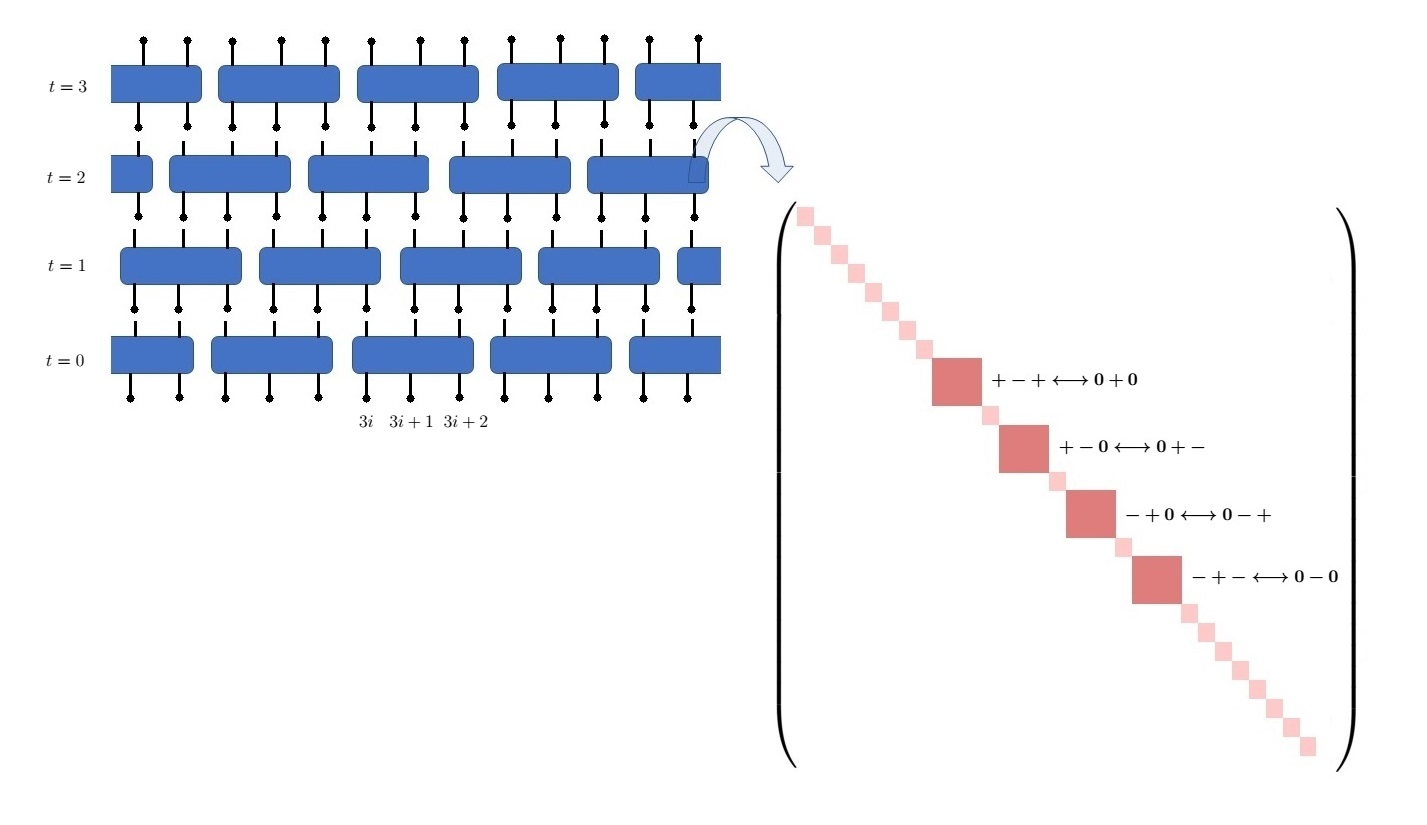
\includegraphics[width=.5\textwidth]{PaiArch}
	\caption{Architecture of the 3-site gate circuit. Each gate is a matrix of the form on the right, where each square is independently chosen from the applicable Haar distribution. The matrix is very sparse, corresponding to the small number of possible transitions. There are 4, as in Tab.~\ref{tab:pai} after adding the negative charge states. Figure from~\cite{PaiFracton}.}
	\label{fig:PaiArch}
\end{figure}
This architecture results in asymmetric lightcone velocities, but we will only look at spreading in one direction, so that will not be an issue.

\subsection{Behavior of fracton charge} \label{sub:fraccharge}

The first question is simply whether the charges are localized. Ref.~\cite{PaiFracton} starts with a state (not an operator) that has a single charge. 
Recall that positive charge is represented by the $+1$ eigenstate of $Z$. Therefore the state with an initially local fracton is one where $\ex{Z_i}=0$ for all $i$, except for one site $j$ where $\ex{Z_j}=1$. We will choose $j=3$.
The evolution of $\ex{Z_i}(t)$ is shown in Fig~\ref{fig:PaiSzPeak}.
\begin{figure}
	\centering
	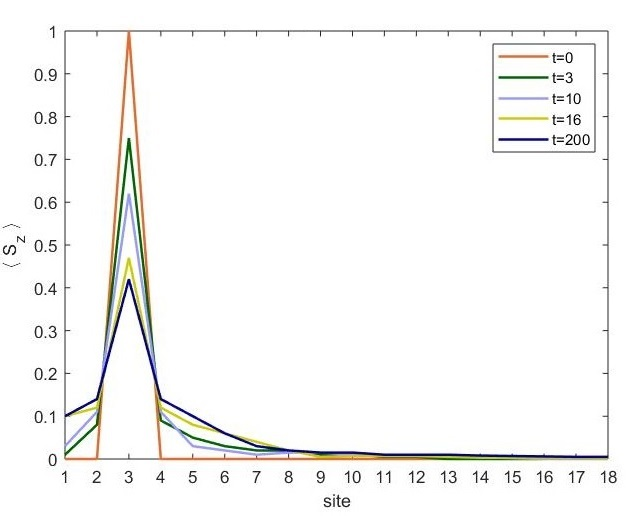
\includegraphics[width=.5\textwidth]{PaiSzPeak}
	\caption{Fracton charge density over time. Note that the fracton peak is not significantly lower at $t=200$ than at $t=16$. Figure from~\cite{PaiFracton}}
	\label{fig:PaiSzPeak}
\end{figure}
The asymptotic value of $\ex{Z_3}$ appears to be $\sim0.4$, so some of the charge does flow. This is a numerical simulation so the results cannot be extended to infinite time, but there does not appear to be significant change between $t=200$ and $t=16$.

Since we cannot perfectly demonstrate the localization of charge out to $t=\infty$, we will make more predictions of the behavior of the fractons in continuous time and space before showing that they match numeric simulations for a fractonic quantum circuit with discrete time and space. In Sec~\ref{sub:fracopsp} we predict operator spreading behavior and show that the numerics match the predictions. Hopefully the combined analysis convinces the reader that the circuits truly manifest localization.

Start by recalling that fractons (charges) are indeed mobile, but dipole conservation requires that the movement of a fracton is paired with the creation of a dipole. These dipoles are then free to move, and in fact they diffuse randomly (hence our previous discussion of diffusion). Say the fracton, with unit negative charge, starts at the origin, and call its position $R$. Since we are in $d=1$, quantities like position and dipole strength will be scalars.\footnote{We will only analyze $d=1$ systems, but Ref.~\cite{PaiFracton} includes calculations for general $d$.}

Consider the creation of a single dipole of magnitude $R$. In $d=1$, a random walk returns to the origin in time $\sim D$.  When the dipole returns to the location of the fracton, the fracton reabsorbs the dipole, returning to the origin. Thus in $d=1$ the fracton stays near the origin, constantly emitting and reabsorbing dipoles. We can think of this situation as a diffusing dipole field, with the fracton acting as a source and sink. This results in the equation
\begin{align}
\pd{\eta}{t}(x) = D\pdn{\eta(x)}{x}{2} + \nd{R}{t}\delta(x-R),
\end{align}
where $\eta$ is the local dipole density.

If initially the fracton is at the origin and no dipoles are present, then the total dipole required to balance out the charge is $\tilde{\eta}=R$. The dipole density at the location of the fracton is $\eta = \tilde{\eta}/\xi$. Thus the fracton equation of motion is
\begin{align}
\nd{R}{t} &= -\eta(R) + A(t)\\
&= \frac{-R}{\sqrt{\pi} DC}+ A(t),
\end{align}
where $A(t)$ is a random force satisfying $\ex{A(t)A(t')} = 2T\delta(t-t')$. \note{The units are very wonky here.} This is a Langavin equation~\cite{MarenduAsp}. The probability distribution for the fracton to be distance $R$ from the origin has solution
\begin{align}
P(R) \sim \exp\left(\frac{R^2}{2\sqrt{\pi}DCT}\right), \label{eqn:lange}
\end{align}
where $T$ is the strength of the random force. 

There are two useful prediction from~(\ref{eqn:lange}. The first is that the tails of fracton density away from the origin (but within the operator spreading front) should take the form of Eq.~\ref{eqn:lange} at late time. Second, as in Eq.~\ref{eqn:lange}, the correlation length of fracton density should scale as $\xi_\text{fracton}\sim \sqrt{DT}$ as the diffusion constant and force strength change. 

To verify these predictions, we once again evolve a state that initially has a single charge on site $i=3$. Then we just have to show that at late time $\ex{Z_i}\sim\exp(R^2/2\sqrt{\pi}DCT)$, $|i-3|=R$. 
In Fig.~\ref{fig:PaiSz} we show a plot of charge density at large $t$. 
\begin{figure}
	\centering
	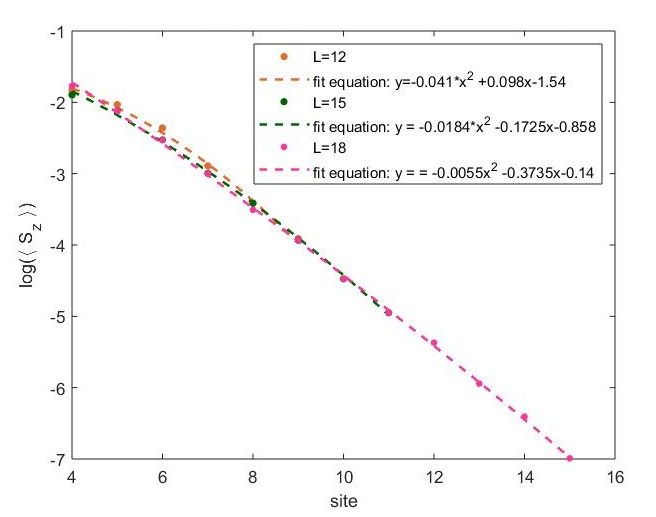
\includegraphics[width=.46\textwidth]{PaiSz}
	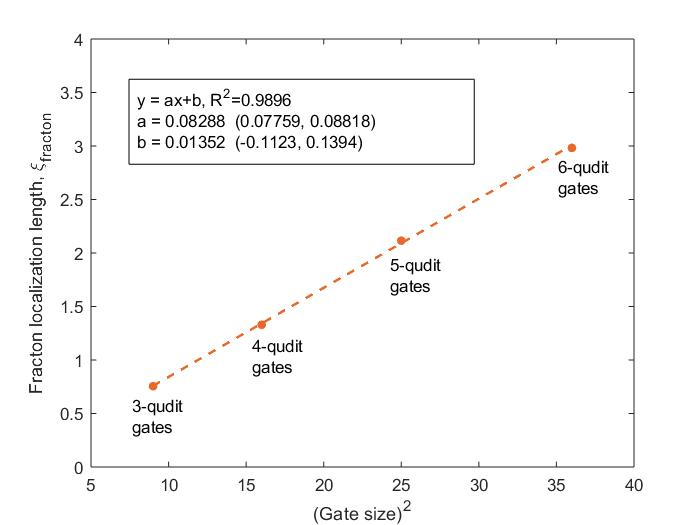
\includegraphics[width=.49\textwidth]{PaiLocLen}
	\caption{Left: Charge density at late times. If $\ex{Z_i}\sim\exp(-x^2)$, then this curve should be quadratic. It cannot be distinguished from a linear function, but the quadratic dependence is not ruled out. Right: Dependence of $\xi_\text{fracton}$ on gate size. This plot more strongly confirms the second prediction of Sec.~\ref{sub:analytic}.}
	\label{fig:PaiSz}
\end{figure}
The exponential dependence means that we can not distinguish between $\exp(-x^2)$ and $\exp(-x)$, so we count the first prediction as a maybe. 

The second prediction also depends on the spreading of charge in a single fracton state. Here, however, we have to be able to change the diffusion constant $D$ and random force $T$. We don't have many parameters left to vary in our system (the circuit is minimally structured) except for gate size. Ref.~\cite{PaiFracton} shows that both $D$ and $T$ scale as $(\text{gate size})^2$, so the second prediction reduces to
\begin{align}
\xi_\text{fracton}\sim\sqrt{DT}\sim(\text{gate size})^2.
\end{align}
$\xi_\text{fracton}$ can be extracted from the late-time charge density, as the half width at half maximum of the charge density peak.
Fig.~\ref{fig:PaiSz} also shows this relationship, confirming this prediction.

\subsection{Operator spreading in fracton circuits} \label{sub:fracopsp}

We once again start by looking at basic localization. That can be shown by starting with an initially local fracton operator (not state) and calculating its evolution. The chosen operator is $IZIII\dots$, where the only non-identity operator is on site 2. Recall that these are spin-1 systems, so 
\begin{align}
Z = \begin{pmatrix} 1 & 0 & 0 \\ 0 & 0 & 0 \\ 0 & 0 & -1 \end{pmatrix}.
\end{align}
The right-weight for this operator is shown in Fig.~\ref{fig:PaiChargeOp}.
\begin{figure}
	\centering
	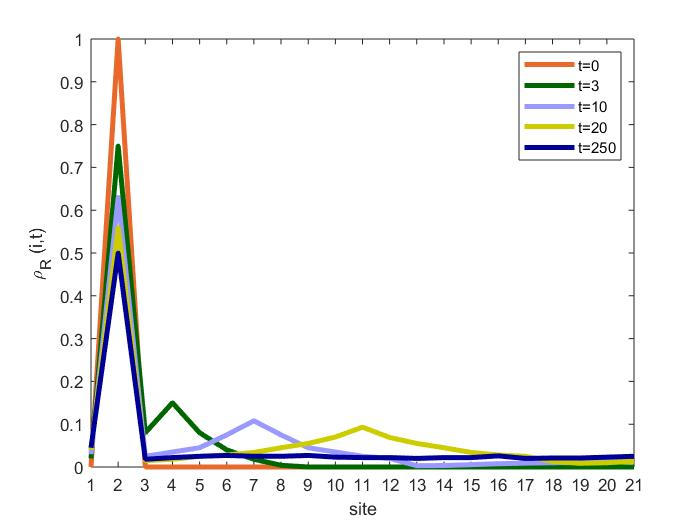
\includegraphics[width=.49\textwidth]{PaiChargeOp}
	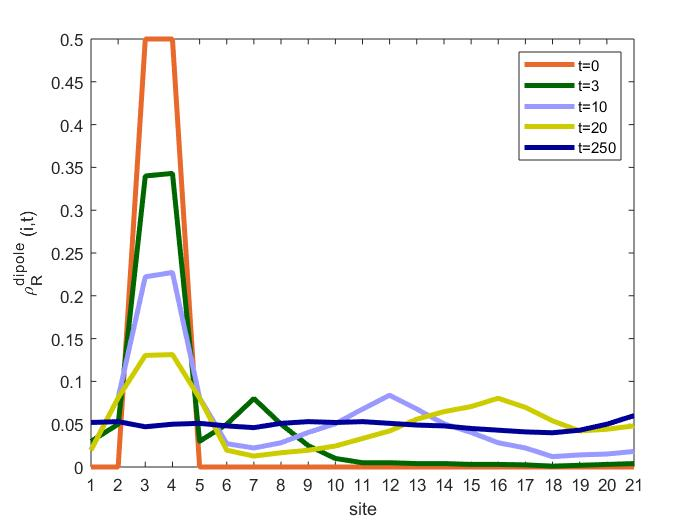
\includegraphics[width=.49\textwidth]{PaiDipoleOp}
	\caption{Operator spreading of the fracton operator and dipole operator, in a 21-site system with open boundary conditions. For the fracton, note the persistent peak at site 2, along with the propagating front. The dipole charge also has a propagating front, but the peak is nonexistent at late time. Figures from~\cite{PaiFracton}}
	\label{fig:PaiChargeOp}
\end{figure}
Note how similar the decrease of $\rho_R(2,t)$ is to $\ex{Z_3}(t)$ in Fig~\ref{fig:PaiSzPeak}.

This is in contrast to the evolution of an initially local dipole operator. Such an operator should be the sum of adjacent fracton operators, so that its eigenstates have positive charge at one state and negative charge at the next. The chosen operator in this case is 
\begin{align}
\th{2}\left(IZIII\dots \vphantom{j}-IIZII\dots\right)
\end{align}
\note{Shouldn't it be $\th{\sqrt{2}}$?} The initial $\th{2}$ ensures that $\sum_i\rho_R(i)=1$. The time evolution of this operator is also shown in Fig.~\ref{fig:PaiChargeOp}. Note that at late time $\sum_i\rho_R(i, t)$ is essentially flat. This shows that the dipole operator is not localized, and suggests further that the late-time behavior of the fracton operator is true localization. 

So far we have focused on the lumps of the spreading operators. The next step is to study the fronts and tails. Since the dipole density behaves like a simple conserved charge, its operator spreading should look like that in Sec.~\ref{sec:cons}. In particular, for an initially local dipole operator, there should be a linearly propagating front that broadens as $\sqrt{t}$, with a power-law tail behind the front. As in Sec~\ref{sec:cons}, the exponent for this tail is $-3/2$.

The spreading of an initially local fracton operator shares the universal structure. There is a lump at the origin corresponding to fracton operators, along with another lump at the origin corresponding to dipole operators. The dipole operators are emitted by the fracton operators in the same way that nonconserved operators are emitted by conserved operators in Sec~\ref{sec:cons}. However, since the dipole operators are also conserved, they do not propagate ($v_{B, \text{dipole}}=0$) and this dipole lump remains at the origin.

The dipole operators at the origin have amplitude~\cite{PaiFracton}
\begin{align}
a^c(x,t) \sim \frac{x}{t^{3/2}}e^{-x^2/Dt}
\end{align}
so the total weight in the dipole lump is
\begin{align}
\rho^c_\tot(t) \sim \int dx\,\abs{a^c(x,t} \sim t^{-3/2}. \label{eqn:fraclump}
\end{align}
This is confirmed in Fig~\ref{fig:PaiFracLump}.
\begin{figure}
	\centering
	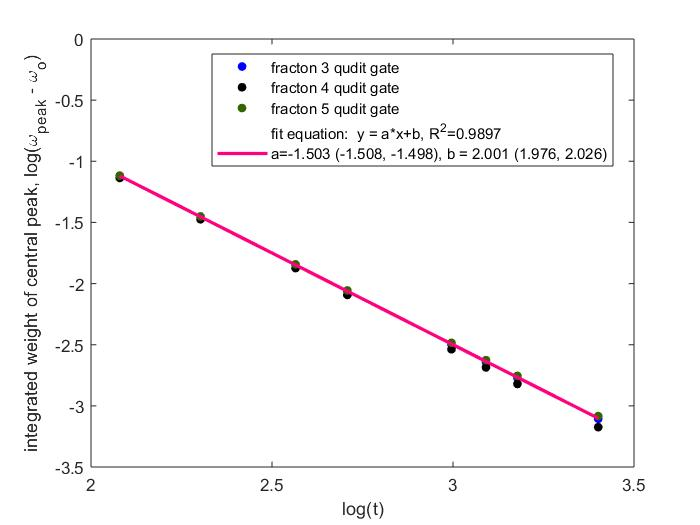
\includegraphics[width=.5\textwidth]{PaiFracLump}
	\caption{Total operator weight in the central lump (or peak) of the conserved dipole operators. The lump is defined as the original site plus the two on each side. We are only interested in the 3-site gate circuit. Figure from~\cite{PaiFracton}}
	\label{fig:PaiFracLump}
\end{figure}
The conserved operator lump in Sec.~\ref{sub:ccons} decreased $\sim t^{-1/2}$, and~(\ref{eqn:powtail}) showed that this made the tail of $\rho_R^\nc(x,t)\sim (t-x/v_B)^{-3/2}$. For the fracton circuit, we have
\begin{align}
\rho_R^\nc(x,t)\sim\pd{\rho_\tot^c(t-x/v_B)}{t} \sim\th{(t-x/v_B)^{5/2}}. 
\end{align}
Thus another prediction to check for the fracton circuit is the different exponents for the power-law tails in the operator right-weights of dipole and fracton operators.

Fig.~\ref{fig:PaiTails} shows some diagnostics for the shape of the spreading dipole and fracton operators. In both cases the front broadens diffusively because the operators in the front are non-conserved operators performing a biased random walk. We can also look at the power-law tails for both types of operators at various times. In all cases, the best-fit exponents closely match $-3/2$ and $-5/2$.
\begin{figure}
	\centering
	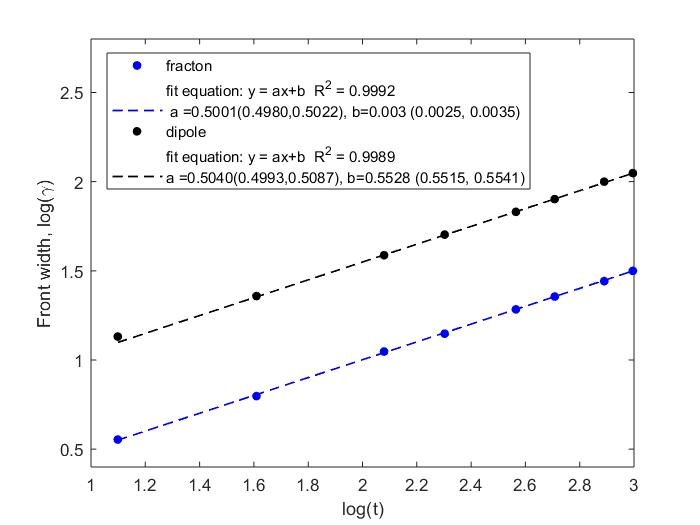
\includegraphics[width=.51\textwidth]{PaiFronts}
	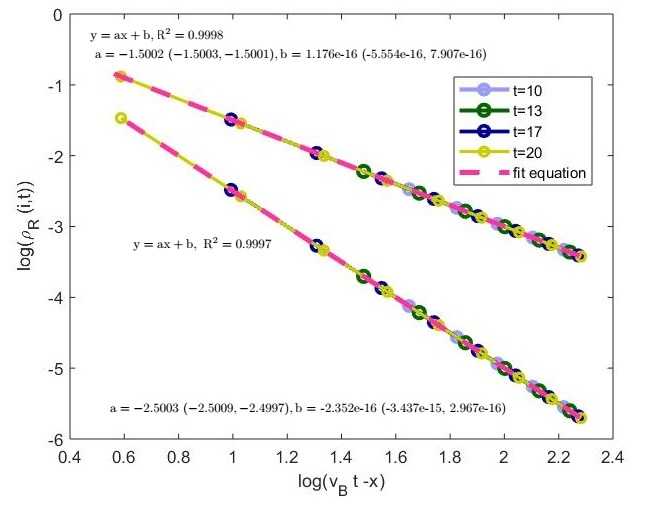
\includegraphics[width=.47\textwidth]{PaiTails}
	\caption{Behavior of the operator right weight at and behind the front. 
		On the left we see that the operator fronts broaden as $\sqrt{t}$ for both fracton and dipole operators, just as in the case of the charge-conserving circuit.
		On the right we see the behavior of the tails behind the fronts. Each color plots the power-law tail behind the front at constant time. The tails at different times are rescaled to lie on the same line (but the exponents are not changed). For the dipole operator, $\rho_R$ decreases with exponent $-3/2$ as in Sec.~\ref{sec:cons}. For the fracton operator the exponent is $-5/2$ instead. }
	\label{fig:PaiTails}
\end{figure}


\section{Results and Conclusions} \label{sec:conc}

The purpose of this essay has been to introduce the reader to quantum dynamics, convince the reader that random unitary circuits are a useful tool in the analysis of dynamics, and show that a certain class of circuits provide a useful model of localization. Along the way is has\dots


%%%%%%%%%%%%%%%%%%%%%%%%%%%%%%%%%%%%%%%%%%%%%%%%%%%%%%%%%%%%%%%%%%
%\printbibliography
%%%%%%%%%%%%%%%%%%%%%%%%%%%%%%%%%%%%%%%%%%%%%%%%%%%%%%%%%%%%%%%%%%
\nocite{apsrev41Control}
\bibliography{../global,revtex-custom}
%%%%%%%%%%%%%%%%%%%%%%%%%%%%%%%%%%%%%%%%%%%%%%%%%%%%%%%%%%%%%%%%%%

\end{document}
